\newpage
\subsection{QuizziPedia::Front-End::Controllers}


\begin{figure} [ht]
	\centering
	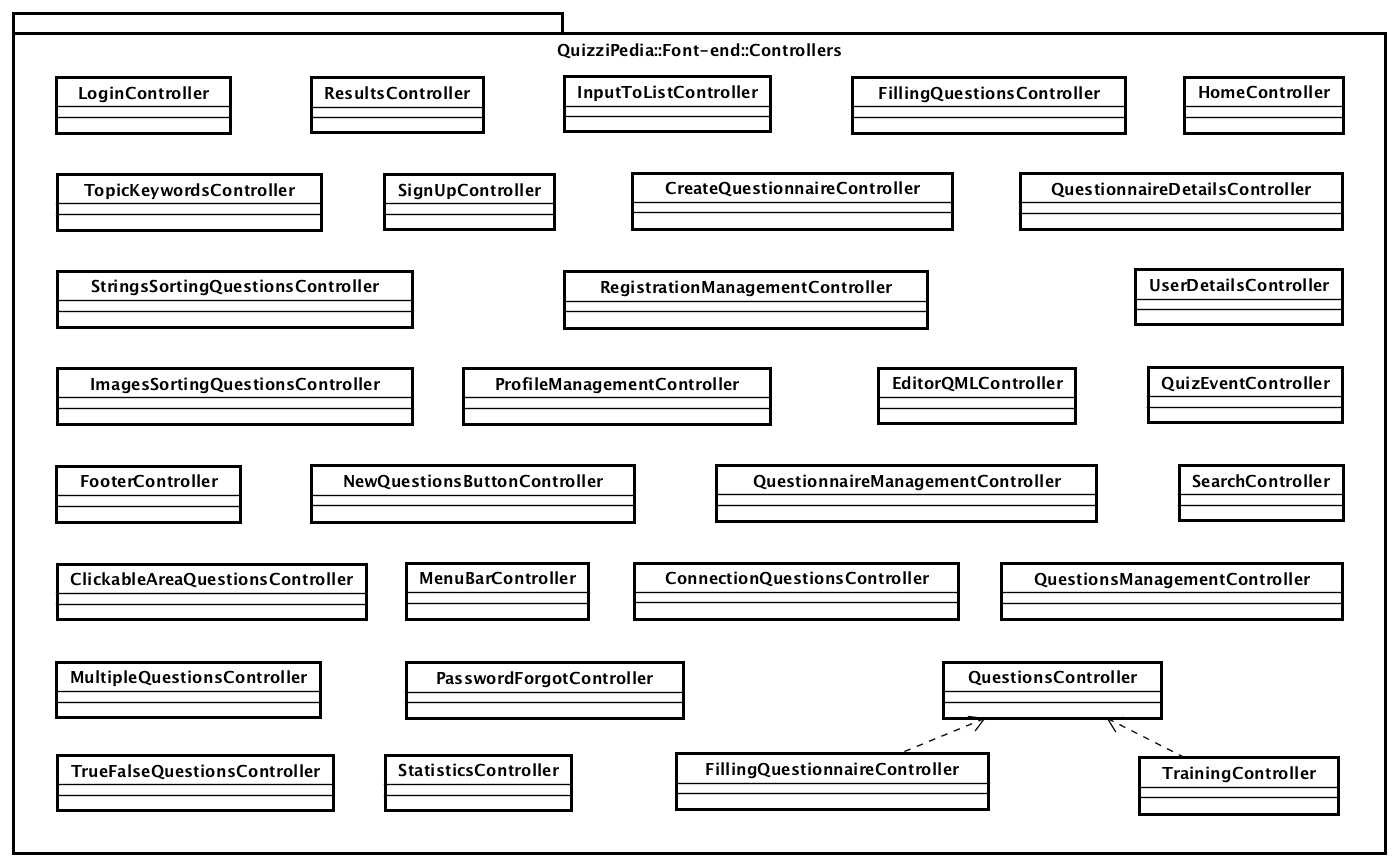
\includegraphics[scale=0.45]{UML/Package/QuizziPedia_Front-End_Controllers.png}
	\caption{QuizziPedia::Front-End::Controllers}
\end{figure} \FloatBarrier

\subsubsection{Informazioni generali}
\begin{itemize}
	\item \textbf{Descrizione}: package che contiene i controller individuati per la parte front-end dell'applicazione;
	\item \textbf{Padre}: \texttt{Front-End};
	\item \textbf{Interazione con altri componenti}:
	\begin{itemize}
		\item \texttt{Models}: package che contiene le classi model individuate;
		\item \texttt{Services}: package che contiene le classi services individuate.
	\end{itemize} 
\end{itemize}
\subsubsection{Classi}

\paragraph{QuizziPedia::Front-End::Controllers::LoginController}
\begin{figure} [ht]
	\centering
	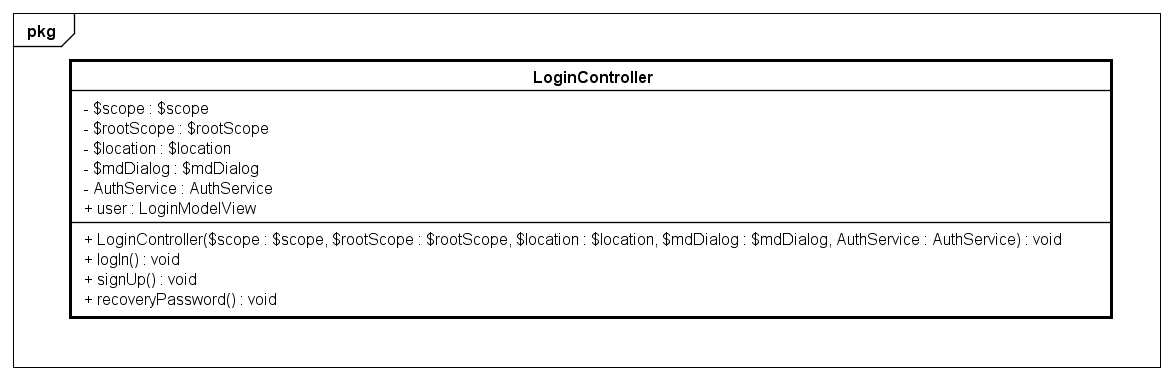
\includegraphics[scale=0.45]{UML/Classi/Front-End/QuizziPedia_Front-end_Controller_LoginController.png}
	\caption{QuizziPedia::Front-End::Controllers::LoginController}
\end{figure} \FloatBarrier
\begin{itemize}
	\item \textbf{Descrizione}: questa classe permette di gestire l'autenticazione dell'utente al sistema; 
	\item \textbf{Utilizzo}: fornisce le funzionalità di autenticazione al sistema, compresa la gestione di situazioni di errore autenticazione;
	\item \textbf{Relazione con altre classi}:
	\begin{itemize}
		\item \textit{OUT} \texttt{LoginModelView}: classe di tipo modelview la cui istanzazione è contenuta all'interno della variabile di ambiente \$scope di \texttt{Angular.js}. All'interno di essa sono presenti le variabili e i metodi necessari per il \textit{Two-Way Data-Binding\ped{G}} tra la view \texttt{LoginView} e il controller \texttt{LoginController};
		\item \textit{IN} \texttt{AuthService}: questa classe permette di gestire la registrazione e l'autenticazione di un utente;
	\end{itemize}
	\item \textbf{Attributi}:
	\begin{itemize}
		\item \texttt{-} \texttt{\$scope: \$scope} \\
		Campo dati contenente un riferimento all’oggetto \$scope creato da \textit{Angular\ped{G}}. Viene utilizzato come mezzo di comunicazione tra il controller e la view. Contiene gli oggetti che definiscono il viewmodel e il model dell’applicazione;
		\item \texttt{-} \texttt{\$rootScope: \$rootScope} \\
		Campo dati contenente il riferimento all'oggetto globale \$rootScope creato da \textit{Angular\ped{G}}. Viene utilizzato per rendere accessibile a tutti i controller e a tutte le view l'oggetto \texttt{UserDetailsModel}. Nel caso della login viene utilizzato per inserire in \$rootScope l'oggetto di ritorno della chiamata a \texttt{logIn()} del service \texttt{AuthService} di tipo \texttt{UserDetailsModel};
		\item \texttt{-} \texttt{\$location: \$location} \\
		Campo dati contenente un riferimento al servizio creato da \textit{Angular\ped{G}} che permette di accedere alla barra degli indirizzi del \textit{browser\ped{G}}, i cambiamenti all’URL nella barra degli indirizzi si riflettono in questo oggetto e viceversa;
		\item \texttt{-} \texttt{\$mdDialog: \$mdDialog} \\
		Campo dati contenente un riferimento al servizio della libreria \textit{Material for Angular\ped{G}} che permette di creare delle componenti a popup;
		\item \texttt{-} \texttt{AuthService: AuthService} \\
		Campo dati contenente un riferimento al servizio che si occupa della gestione delle informazioni legate all’autenticazione. Viene utilizzato il metodo \texttt{logIn} di \$texttt{AuthService} a cui vengono passati i parametri \texttt{username} e \texttt{password};
		\item \texttt{+} \texttt{user: LoginModelView} \\
		Oggetto di tipo \texttt{LoginModelView}. All'interno di esso sono presenti le variabili e i metodi necessari per il \textit{Two-Way Data-Binding\ped{G}} tra la view \texttt{LoginView} e il controller \texttt{LoginController};
	\end{itemize}
	\item \textbf{Metodi}:
	\begin{itemize}
		\item \texttt{+} \texttt{LoginController(\$scope: \$scope, \$rootScope: \$rootScope, \$location: \$location, \$mdDialog: \$mdDialog, AuthService: AuthService)} \\
		Metodo costruttore della classe; \\
		\textbf{Parametri}:
			\begin{itemize}
				\item \texttt{\$scope: \$scope} \\
				Parametro contenente un riferimento all’oggetto \$scope creato da \textit{Angular\ped{G}}. Viene utilizzato come mezzo di comunicazione tra il controller e la view. Contiene gli oggetti che definiscono il viewmodel e il model dell’applicazione;
				\item \texttt{\$rootScope: \$rootScope} \\
				Parametro contenente il riferimento all'oggetto globale \$rootScope creato da \textit{Angular\ped{G}}. Viene utilizzato per rendere accessibile a tutti i controller e a tutte le view l'oggetto \texttt{UserDetailsModel}. Nel caso della login viene utilizzato per inserire in \$rootScope l'oggetto di ritorno della chiamata a \texttt{logIn()} del service \texttt{AuthService};
				\item \texttt{\$location: \$location} \\
				Parametro contenente un riferimento al servizio creato da \textit{Angular\ped{G}} che permette di accedere alla barra degli indirizzi del \textit{browser\ped{G}}, i cambiamenti all’URL nella barra degli indirizzi si riflettono in questo oggetto e viceversa;
				\item \texttt{\$mdDialog: \$mdDialog} \\
				Parametro contenente un riferimento al servizio della libreria \textit{Material for Angular\ped{G}} che permette di creare delle componenti a popup;
				\item \texttt{AuthService: AuthService} \\
				Campo dati contenente un riferimento al servizio che si occupa della gestione delle informazioni legate all’autenticazione. Viene utilizzato il metodo \texttt{logIn} di \$texttt{AuthService} a cui vengono passati i parametri \texttt{username} e \texttt{password};
			\end{itemize}
		\item \texttt{+} \texttt{logIn(): void} \\
		Metodo che richiama il metodo \texttt{Login} del service \texttt{AuthService} passandogli \texttt{username} e \texttt{password}. Nel caso di buona riuscita dell'operazione, viene inserito nell'oggetto globale \texttt{\$rootScope} l'utente corrente che ha come model l'\texttt{UserDetailsModel} e poi viene effettuato il redirect alla homepage dell'applicazione. Nel caso in cui invece avvenga un errore, viene mostrato a video il messaggio di errore;
		\item \texttt{+} \texttt{signUp(): void} \\
		Metodo che gestisce l’evento click sul pulsante di registrazione. Effettua il redirect alla pagina di registrazione;
		\item \texttt{+} \texttt{recoveryPassword(): void} \\
		Metodo che gestisce l’evento click sul pulsante di recupero password. Effettua il redirect alla pagina per il recupero della password; 
	\end{itemize}
\end{itemize}

\paragraph{QuizziPedia::Front-End::Controllers::SignUpController}
\begin{figure} [ht]
	\centering
	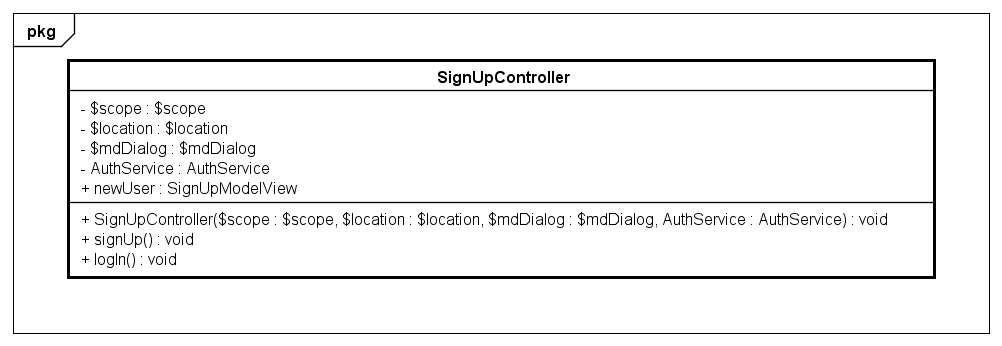
\includegraphics[scale=0.45]{UML/Classi/Front-End/QuizziPedia_Front-end_Controller_SignUpController.png}
	\caption{QuizziPedia::Front-End::Controllers::SignUpController}
\end{figure} \FloatBarrier
\begin{itemize}
	\item \textbf{Descrizione}: questa classe permette di gestire la registrazione di un utente al sistema;
	\item \textbf{Utilizzo}: fornisce le funzionalità di registrazione di un utente al sistema;
	\item \textbf{Relazione con altre classi}:
	\begin{itemize}
		\item \textit{IN} \texttt{SignUpModelView}: classe di tipo modelview la cui istanzazione è contenuta all'interno della variabile di ambiente \$scope di \texttt{Angular.js}. All'interno di essa sono presenti le variabili e i metodi necessari per il \textit{Two-Way Data-Binding\ped{G}} tra la view \texttt{SignUpView} e il controller \texttt{SignUpController};
		\item \textit{IN} \texttt{AuthService}: questa classe permette di gestire la registrazione e l'autenticazione di un utente;
	\end{itemize}
	\item \textbf{Attributi}:
	\begin{itemize}
		\item \texttt{-} \texttt{\$scope: \$scope} \\
		Campo dati contenente un riferimento all’oggetto \$scope creato da \textit{Angular\ped{G}}. Viene utilizzato come mezzo di comunicazione tra il controller e la view. Contiene gli oggetti che definiscono il viewmodel e il model dell’applicazione;
		\item \texttt{-} \texttt{\$location: \$location} \\
		Campo dati contenente un riferimento al servizio creato da \textit{Angular\ped{G}} che permette di accedere alla barra degli indirizzi del \textit{browser\ped{G}}, i cambiamenti all’URL nella barra degli indirizzi si riflettono in questo oggetto e viceversa;
		\item \texttt{-} \texttt{\$mdDialog: \$mdDialog} \\
		Campo dati contenente un riferimento al servizio della libreria \textit{Material for Angular\ped{G}} che permette di creare delle componenti a popup;
		\item \texttt{-} \texttt{AuthService: AuthService} \\
		Campo dati contenente un riferimento al servizio che si occupa della gestione delle informazioni legate all’autenticazione. Viene utilizzato il metodo \texttt{signUp} di \$texttt{AuthService} a cui viene passato come parametro un oggetto di tipo \texttt{SignUpModelView};
		\item \texttt{+} \texttt{newUser: SignUpModelView} \\
		Oggetto di tipo \texttt{SignUpModelView}. All'interno di esso sono presenti le variabili e i metodi necessari per il \textit{Two-Way Data-Binding\ped{G}} tra la view \texttt{SignUpView} e il controller \texttt{SignUpController};
	\end{itemize}
	\item \textbf{Metodi}:
	\begin{itemize}
		\item \texttt{+} \texttt{SignUpController(\$scope: \$scope, \$location: \$location, \$mdDialog: \$mdDialog, AuthService: AuthService)} \\
		Metodo costruttore della classe; \\
		\textbf{Parametri}:
		\begin{itemize}
			\item \texttt{\$scope: \$scope} \\
			Parametro contenente un riferimento all’oggetto \$scope creato da \textit{Angular\ped{G}}. Viene utilizzato come mezzo di comunicazione tra il controller e la view. Contiene gli oggetti che definiscono il viewmodel e il model dell’applicazione;
			\item \texttt{\$location: \$location} \\
			Parametro contenente un riferimento al servizio creato da \textit{Angular\ped{G}} che permette di accedere alla barra degli indirizzi del \textit{browser\ped{G}}, i cambiamenti all’URL nella barra degli indirizzi si riflettono in questo oggetto e viceversa;
			\item \texttt{\$mdDialog: \$mdDialog} \\
			Parametro contenente un riferimento al servizio della libreria \textit{Material for Angular\ped{G}} che permette di creare delle componenti a popup;
			\item \texttt{AuthService: AuthService} \\
			Campo dati contenente un riferimento al servizio che si occupa della gestione delle informazioni legate all’autenticazione. Viene utilizzato il metodo \texttt{logIn} di \$texttt{AuthService} a cui vengono passati i parametri \texttt{username} e \texttt{password};
		\end{itemize}
		\item \texttt{+} \texttt{signUp(): void} \\
		Metodo che richiama il metodo \texttt{signUp} del service \texttt{AuthService} passandogli un oggetto di tipo \texttt{SignUpModelView}. Nel caso di buona riuscita dell'operazione viene mostrato un messaggio di successo. Con l'azione di click sul bottone presentato dal messaggio di successo è possibile effettuare il redirect alla pagina di login dell'applicazione. Nel caso in cui invece avvenga un errore, viene mostrato a video il messaggio di errore;
		\item \texttt{+} \texttt{logIn(): void} \\
		Metodo che gestisce l’evento click sul pulsante di login. Effettua il redirect alla pagina di login;
	
	\end{itemize}
\end{itemize}

\paragraph{QuizziPedia::Front-End::Controllers::HomeController}
\begin{figure} [ht]
	\centering
	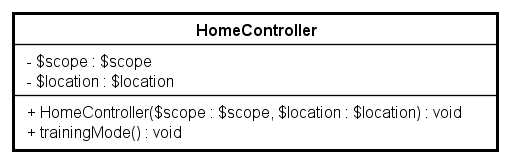
\includegraphics[scale=0.45]{UML/Classi/Front-End/QuizziPedia_Front-end_Controller_HomeController.png}
	\caption{QuizziPedia::Front-End::Controllers::HomeController}
\end{figure} \FloatBarrier
\begin{itemize}
	\item \textbf{Descrizione}: questa classe permette di gestire la home page;
	\item \textbf{Utilizzo}: fornisce tutte le informazioni da mostrare nella homepage;
	\item \textbf{Relazione con altre classi}:
	\begin{itemize}
		\item \textit{IN} \texttt{HomeModelView}: classe di tipo modelview la cui istanzazione è contenuta all'interno della variabile di ambiente \$scope di \texttt{Angular.js}. All'interno di essa sono presenti le variabili e i metodi necessari per il \textit{Two-Way Data-Binding\ped{G}} tra la view \texttt{HomeView} e il controller \texttt{HomeController};
	\end{itemize}
	\item \textbf{Attributi}:
	\begin{itemize}
		\item \texttt{-} \texttt{\$scope: \$scope} \\
		Campo dati contenente un riferimento all’oggetto \$scope creato da \textit{Angular\ped{G}}, viene utilizzato come mezzo di comunicazione tra il controller e la view. Contiene gli oggetti che definiscono il model dell’applicazione;
		\item \texttt{-} \texttt{\$location: \$location} \\
		Campo dati contenente un riferimento al servizio creato da \textit{Angular\ped{G}} che permette di accedere alla barra degli indirizzi del \textit{browser\ped{G}}, i cambiamenti all’URL nella barra degli indirizzi si riflettono in questo oggetto e viceversa;
	\end{itemize}
	\item \textbf{Metodi}:
	\begin{itemize}
		\item \texttt{+} \texttt{trainingMode(): void} \\
		Metodo che gestisce l’evento click sul pulsante di allenamento. Effettua il redirect alla pagina di allenamento; 
	\end{itemize}
\end{itemize}

\paragraph{QuizziPedia::Front-End::Controllers::SearchController}
\begin{figure} [ht]
	\centering
	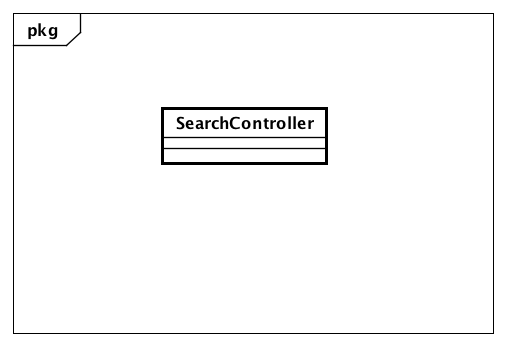
\includegraphics[scale=0.45]{UML/Classi/Front-End/QuizziPedia_Front-end_Controller_SearchController.png}
	\caption{QuizziPedia::Front-End::Controllers::SearchController}
\end{figure} \FloatBarrier
\begin{itemize}
	\item \textbf{Descrizione}: questa classe permette di gestire la ricerca di questionari e utenti all'interno dell'applicazione;
	\item \textbf{Utilizzo}: fornisce all'utente le funzionalità di ricerca per utenti e questionari;
	\item \textbf{Relazione con altre classi}:
	\begin{itemize}
		\item \textit{IN} \texttt{ResultsModelView}: view contenente i risultati della ricerca effettuata, sia gli utenti che i questionari;
		\item \textit{IN} \texttt{SearchService}: questa classe permette di ottenere i dati personali degli utenti;
		\item \textit{IN} \texttt{QuizService}: questa classe permette di ottenere i dati di un quiz tramite delle parole chiave inserite dall'utente nella barra di ricerca;
	\end{itemize}
	\item \textbf{Attributi}:
	\begin{itemize}
		\item \texttt{-} \texttt{\$scope: \$scope} \\
		Campo dati contenente un riferimento all’oggetto \$scope creato da \textit{Angular\ped{G}}, viene utilizzato come mezzo di comunicazione tra il controller e la view. Contiene gli oggetti che definiscono il model dell’applicazione;
		\item \texttt{-} \texttt{\$location: \$location} \\
		Campo dati contenente un riferimento al servizio creato da \textit{Angular\ped{G}} che permette di accedere alla barra degli indirizzi del \textit{browser\ped{G}}, i cambiamenti all’URL nella barra degli indirizzi si riflettono in questo oggetto e viceversa;
		\item \texttt{\$mdDialog: \$mdDialog} \\
		Parametro contenente un riferimento al servizio della libreria \textit{Material for Angular\ped{G}} che permette di creare delle componenti a popup;
		\item \texttt{-} \texttt{SearchService: SearchService} \\
		\item \texttt{-} \texttt{QuizService: QuizService} \\
	\end{itemize}
	\item \textbf{Metodi}:
	\begin{itemize}
		\item \texttt{+} \texttt{SearchController(\$scope: \$scope, \$location: \$location, \$mdDialog: \$mdDialog)} \\
		Metodo costruttore della classe; \\ 
		\item \texttt{-} \texttt{getSearch(stringSearch: String): SearchModelView} \\
		\item \texttt{+} \texttt{goToUser(idUser: String): void} \\
		Evento per andare all'utente;
		\item \texttt{+} \texttt{registrationToQuiz(idQuiz: String): void} \\
		Evento per registrarsi al questionario attraverso quiz service;
	\end{itemize}
\end{itemize}

\paragraph{QuizziPedia::Front-End::Controllers::ProfileManagementController}
\begin{figure} [ht]
	\centering
	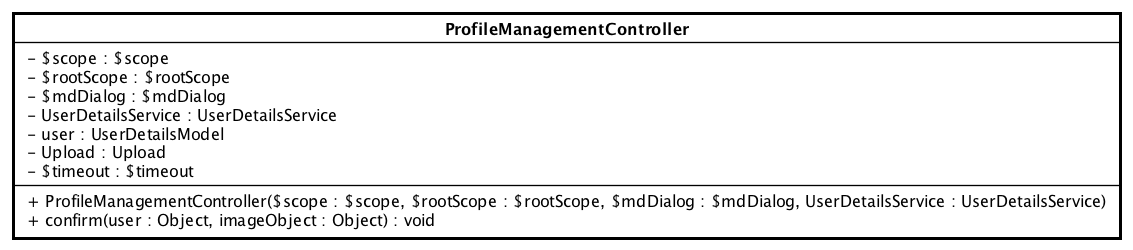
\includegraphics[scale=0.45]{UML/Classi/Front-End/QuizziPedia_Front-end_Controller_ProfileManagementController.png}
	\caption{QuizziPedia::Front-End::Controllers::ProfileManagementController}
\end{figure} \FloatBarrier
\begin{itemize}
	\item \textbf{Descrizione}: questa classe permette di gestire il profilo personale di un utente; 
	\item \textbf{Utilizzo}: fornisce le funzionalità all'utente per poter gestire i propri dati;
	\item \textbf{Relazione con altre classi}:
	\begin{itemize}
		\item \textit{IN} \texttt{ProfileManagementModelView}: ;
		\item \textit{IN} \texttt{UserDetailsService}: questa classe permette di ottenere i dati personali degli utenti;
		\item \textit{IN} \texttt{UserDetailsModel}: 
	\end{itemize}
	\item \textbf{Attributi}:
	\begin{itemize}
		\item \texttt{-} \texttt{\$scope: \$scope} \\
		Campo dati contenente un riferimento all’oggetto \$scope creato da \textit{Angular\ped{G}}, viene utilizzato come mezzo di comunicazione tra il controller e la view. Contiene gli oggetti che definiscono il model dell’applicazione;
		\item \texttt{-} \texttt{\$rootScope: \$rootScope} \\
		Campo dati contenente il riferimento all'oggetto globale \$rootScope creato da \textit{Angular\ped{G}}. Viene utilizzato per rendere accessibile a tutti i controller e a tutte le view l'oggetto \texttt{UserDetailsModel};
		\item \texttt{-} \texttt{\$mdDialog: \$mdDialog} \\
		Campo dati contenente un riferimento al servizio della libreria \textit{Material for Angular\ped{G}} che permette di creare delle componenti a popup;		
		\item \texttt{-} \texttt{UserDetailsService: UserDetailsService}: \\
	\end{itemize}
	\item \textbf{Metodi}:
	\begin{itemize}
		\item \texttt{ProfileManagementController}: \\Metodo costruttore della classe
		\item \texttt{getuserDetails}: \\
		\item \texttt{+} \texttt{confirm(): void} \\
		Metodo che gestisce l’evento click sul pulsante di conferma modifica. Gestisce l'invio dei nuovi oggetti creati al back-end per il salvaggio persistente dei dati. Aggiorna inoltre UserDetailsModel.

	\end{itemize}
\end{itemize}

\paragraph{QuizziPedia::Front-End::Controllers::LogoutController}
\begin{figure} [ht]
	\centering
	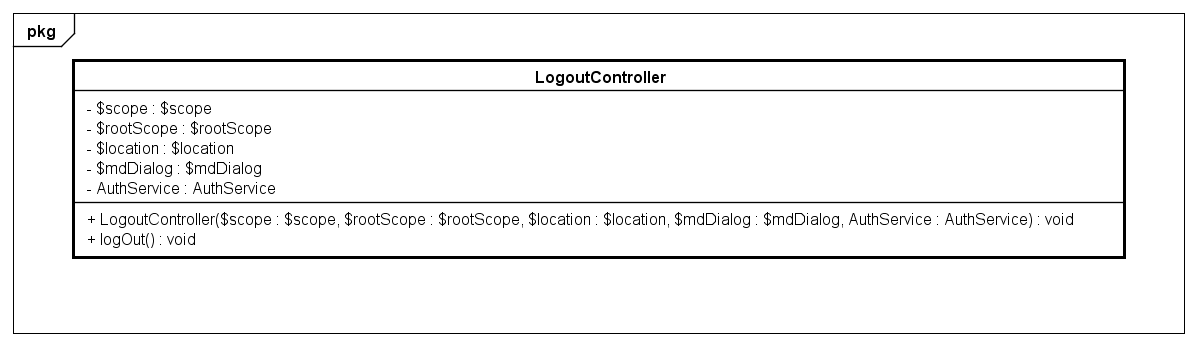
\includegraphics[scale=0.45]{UML/Classi/Front-End/QuizziPedia_Front-end_Controller_LogoutController.png}
	\caption{QuizziPedia::Front-End::Controllers::LogoutController}
\end{figure} \FloatBarrier
\begin{itemize}
	\item \textbf{Descrizione}: questa classe permette di gestire l'azione di logout;
	\item \textbf{Utilizzo}: fornisce la funzionalità per effettuare il logout dall'applicazione;
	\item \textbf{Relazione con altre classi}:
	\begin{itemize}
		\item \textit{OUT} \texttt{MenuBarDirective}: rappresenta il menù, presente in ogni pagina dell'applicazione, generato in base agli oggetti passati nello \$scope isolato. Fornisce un pulsante per ogni oggetto ricevuto come parametro, ogni pulsante viene rappresentato con un’icona e con un testo. Al click di un pulsante viene invocata la funzione ad esso associata. Nel caso di un utente autenticato sarà presente un bottone per effettuare il logout;
		\item \textit{IN} \texttt{AuthService}: questa classe permette di gestire la registrazione e l'autenticazione di un utente;
	\end{itemize}
	\item \textbf{Attributi}:
	\begin{itemize}
		\item \texttt{-} \texttt{\$scope: \$scope} \\
		Campo dati contenente un riferimento all’oggetto \$scope creato da \textit{Angular\ped{G}}. Viene utilizzato come mezzo di comunicazione tra il controller e la view. Contiene gli oggetti che definiscono il viewmodel e il model dell’applicazione;
		\item \texttt{-} \texttt{\$rootScope: \$rootScope} \\
		Campo dati contenente il riferimento all'oggetto globale \$rootScope creato da \textit{Angular\ped{G}}. Viene utilizzato per rendere accessibile a tutti i controller e a tutte le view l'oggetto \texttt{UserDetailsModel}. Nel caso della logout viene utilizzata per rimuovere da \$rootScope l'oggetto di di tipo \texttt{UsersDetailModel};
		\item \texttt{-} \texttt{\$location: \$location} \\
		Campo dati contenente un riferimento al servizio creato da \textit{Angular\ped{G}} che permette di accedere alla barra degli indirizzi del \textit{browser\ped{G}}, i cambiamenti all’URL nella barra degli indirizzi si riflettono in questo oggetto e viceversa;
		\item \texttt{-} \texttt{\$mdDialog: \$mdDialog} \\
		Campo dati contenente un riferimento al servizio della libreria \textit{Material for Angular\ped{G}} che permette di creare delle componenti a popup;
		\item \texttt{-} \texttt{AuthService: AuthService} \\
		Campo dati contenente un riferimento al servizio che si occupa della gestione delle informazioni legate all’autenticazione. Viene utilizzato il metodo \texttt{logOut} di \$texttt{AuthService} a cui viene passato il parametro \texttt{username};
	\end{itemize}
	\item \textbf{Metodi}:
	\begin{itemize}
		\item \texttt{+} \texttt{LogoutController(\$scope: \$scope, \$rootScope: \$rootScope, \$location: \$location, \$mdDialog: \$mdDialog, AuthService: AuthService)} \\
		Metodo costruttore della classe; \\
		\textbf{Parametri}:
		\begin{itemize}
			\item \texttt{\$scope: \$scope} \\
			Parametro contenente un riferimento all’oggetto \$scope creato da \textit{Angular\ped{G}}. Viene utilizzato come mezzo di comunicazione tra il controller e la view. Contiene gli oggetti che definiscono il viewmodel e il model dell’applicazione;
			\item \texttt{\$rootScope: \$rootScope} \\
			Parametro contenente il riferimento all'oggetto globale \$rootScope creato da \textit{Angular\ped{G}}. Viene utilizzato per rendere accessibile a tutti i controller e a tutte le view l'oggetto \texttt{UserDetailsModel}. Nel caso della logout viene utilizzata per rimuovere da \$rootScope l'oggetto di di tipo \texttt{UsersDetailModel};
			\item \texttt{\$location: \$location} \\
			Parametro contenente un riferimento al servizio creato da \textit{Angular\ped{G}} che permette di accedere alla barra degli indirizzi del \textit{browser\ped{G}}, i cambiamenti all’URL nella barra degli indirizzi si riflettono in questo oggetto e viceversa;
			\item \texttt{\$mdDialog: \$mdDialog} \\
			Parametro contenente un riferimento al servizio della libreria \textit{Material for Angular\ped{G}} che permette di creare delle componenti a popup;
			\item \texttt{AuthService: AuthService} \\
			Campo dati contenente un riferimento al servizio che si occupa della gestione delle informazioni legate all’autenticazione.  Viene utilizzato il metodo \texttt{logOut} di \$texttt{AuthService} a cui viene passato il parametro \texttt{username};
		\end{itemize}
		\item \texttt{+} \texttt{logOut(): void} \\
		Metodo che richiama il metodo \texttt{logOut} del service \texttt{AuthService} passandogli lo \texttt{username}. Prima di effettuare questa operazione viene mostrato a video un messaggio di conferma per il proseguo dell'operazione;
	\end{itemize}
\end{itemize}

\paragraph{QuizziPedia::Front-End::Controllers::PasswordForgotController}
\begin{figure} [ht]
	\centering
	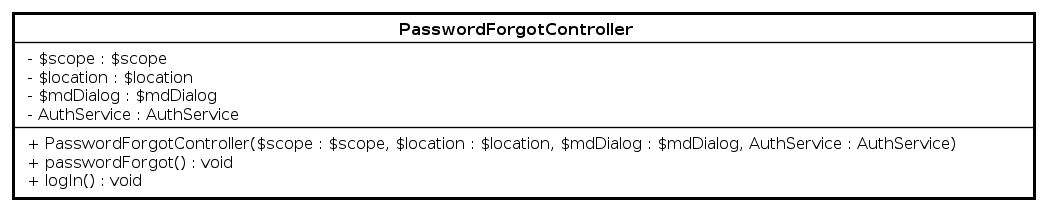
\includegraphics[scale=0.45]{UML/Classi/Front-End/QuizziPedia_Front-end_Controller_PasswordForgotController.png}
	\caption{QuizziPedia::Front-End::Controllers::PasswordForgotController}
\end{figure} \FloatBarrier
\begin{itemize}
	\item \textbf{Descrizione}: questa classe permette di gestire il ripristino della password dimenticata;
	\item \textbf{Utilizzo}: fornisce tutte le funzionalità per ripristinare la password dopo aver verificato l'identità dell'utente;
	\item \textbf{Relazione con altre classi}:
	\begin{itemize}
		\item \textit{IN} \texttt{PasswordForgotModelView}: classe di tipo modelview la cui istanzazione è contenuta all'interno della variabile di ambiente \$scope di \texttt{Angular.js}. All'interno di essa sono presenti le variabili e i metodi necessari per il \textit{Two-Way Data-Binding\ped{G}} tra la view \texttt{PasswordForgotView} e il controller \texttt{PasswordForgotController};
		\item \textit{IN} \texttt{AuthService}: questa classe permette di gestire la registrazione e l'autenticazione di un utente;
	\end{itemize}
	\item \textbf{Attributi}:
	\begin{itemize}
		\item \texttt{-} \texttt{\$scope: \$scope} \\
		Campo dati contenente un riferimento all’oggetto \$scope creato da \textit{Angular\ped{G}}, viene utilizzato come mezzo di comunicazione tra il controller e la view. Contiene gli oggetti che definiscono il model dell’applicazione;
		\item \texttt{-} \texttt{\$location: \$location} \\
		Campo dati contenente un riferimento al servizio creato da \textit{Angular\ped{G}} che permette di accedere alla barra degli indirizzi del \textit{browser\ped{G}}, i cambiamenti all’URL nella barra degli indirizzi si riflettono in questo oggetto e viceversa;
		\item \texttt{-} \texttt{\$mdDialog: \$mdDialog} \\
		Campo dati contenente un riferimento al servizio della libreria \textit{Material for Angular\ped{G}} che permette di creare delle componenti a popup;
		\item \texttt{-} \texttt{AuthService: AuthService} \\
		Campo dati contenente un riferimento al servizio che si occupa della gestione delle informazioni legate all’autenticazione. Viene utilizzato il metodo \texttt{passwordForgot} di \$texttt{AuthService} a cui viene passato il parametro \texttt{email};
	\end{itemize}
	\item \textbf{Metodi}:
	\begin{itemize}
		\item \texttt{+} \texttt{PasswordForgotController(\$scope: \$scope, \$location: \$location, \$mdDialog: \$mdDialog, AuthService: AuthService)} \\
		Metodo costruttore della classe; \\
		\textbf{Parametri}:
		\begin{itemize}
			\item \texttt{\$scope: \$scope} \\
			Parametro contenente un riferimento all’oggetto \$scope creato da \textit{Angular\ped{G}}. Viene utilizzato come mezzo di comunicazione tra il controller e la view. Contiene gli oggetti che definiscono il viewmodel e il model dell’applicazione;
			\item \texttt{\$location: \$location} \\
			Parametro contenente un riferimento al servizio creato da \textit{Angular\ped{G}} che permette di accedere alla barra degli indirizzi del \textit{browser\ped{G}}, i cambiamenti all’URL nella barra degli indirizzi si riflettono in questo oggetto e viceversa;
			\item \texttt{\$mdDialog: \$mdDialog} \\
			Parametro contenente un riferimento al servizio della libreria \textit{Material for Angular\ped{G}} che permette di creare delle componenti a popup;
			\item \texttt{AuthService: AuthService} \\
			Campo dati contenente un riferimento al servizio che si occupa della gestione delle informazioni legate all’autenticazione. Viene utilizzato il metodo \texttt{passwordForgot} di \$texttt{AuthService} a cui viene passato il parametro \texttt{email};
		\end{itemize}
		\item \texttt{+} \texttt{passwordForgot(): void} \\
		Metodo che richiama il metodo \texttt{passwordForgot} del service \texttt{AuthService} passandogli il parametro \texttt{email}. Nel caso di buona riuscita dell'operazione, viene mostrato un messaggio di successo il cui corpo contiene anche un bottone per effettuare il redirect alla pagina di login. Nel caso in cui invece avvenga un errore, viene mostrato a video il messaggio di errore;
		\item \texttt{+} \texttt{logIn(): void} \\
		Metodo che gestisce l’evento click sul pulsante di login. Effettua il redirect alla pagina di login;
	\end{itemize}
\end{itemize}

\paragraph{QuizziPedia::Front-End::Controllers::TrueFalseQuestionsController}
\begin{figure} [ht]
	\centering
	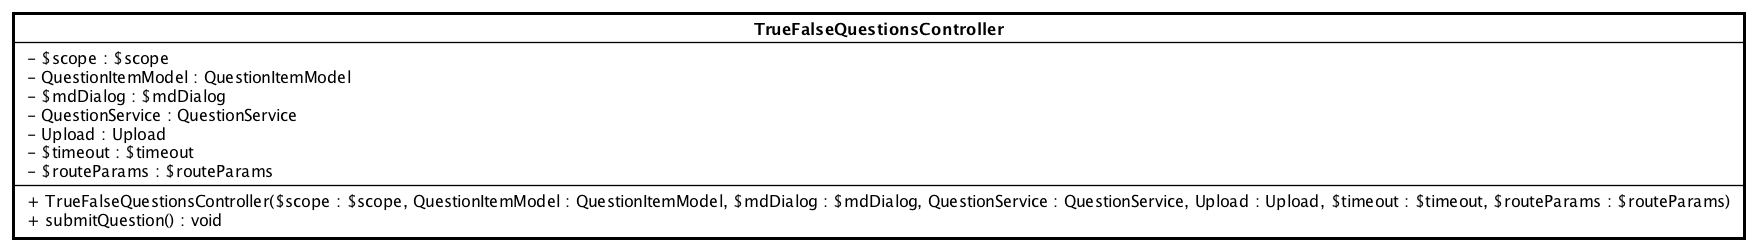
\includegraphics[scale=0.45]{UML/Classi/Front-End/QuizziPedia_Front-end_Controller_TrueFalseQuestionsController.png}
	\caption{QuizziPedia::Front-End::Controllers::TrueFalseQuestionsController}
\end{figure} \FloatBarrier
\begin{itemize}
	\item \textbf{Descrizione}: questa classe permette di gestire la creazione e la modifica di una domanda vero/falso;
	\item \textbf{Utilizzo}: fornisce le funzionalità per inserire una nuova domanda vero/falso nel database e per modificarne una esistente;
	\item \textbf{Relazione con altre classi}:
	\begin{itemize}
		\item \textit{IN} \texttt{TrueFalseQuestionsModelView}: ;
		\item \textit{IN} \texttt{QuestionService}: questa classe permette di ottenere domande esistenti e salvare nuove domande;
		\item \textit{IN} \texttt{QuestionItemModel}: è il modello (astratto) della domanda;
	\end{itemize}
	\item \textbf{Attributi}:
	\begin{itemize}
		\item \texttt{-} \texttt{\$scope: \$scope} \\
		Campo dati contenente un riferimento all’oggetto \$scope creato da \textit{Angular\ped{G}}, viene utilizzato come mezzo di comunicazione tra il controller e la view. Contiene gli oggetti che definiscono il model dell’applicazione;
		\item \texttt{-} \texttt{Question: QuestionItemModel} \\ Oggetto nel quale andremo a salvare la domanda dopo averla scaricata dal service (per poterla caricare nella view);
		\item \texttt{+} \texttt{\$cookie: \$cookie}: serve per recuperare l'id della domanda dalla pagina da cui arrivo;
		\item \texttt{-} \texttt{\$mdDialog: \$mdDialog} \\
		Campo dati contenente un riferimento al servizio della libreria \textit{Material for Angular\ped{G}} che permette di creare delle componenti a popup;
		\item \texttt{-} \texttt{QuestionService: QuestionService}: ;
	\end{itemize}
	\item \textbf{Metodi}:
	\begin{itemize}
		\item \texttt{+} \texttt{TrueFalseQuestionsController} \\ Costruttore della classe (controllerà anche se la domanda esiste (tramite cookie) e in caso la casica, altrimenti view con form vuota);
		\item \texttt{+} \texttt{submitQuestion}: raccoglie i dati dal modelview e li manda al service;
	\end{itemize}
\end{itemize}

\paragraph{QuizziPedia::Front-End::Controllers::MultipleQuestionsController}
\begin{figure} [ht]
	\centering
	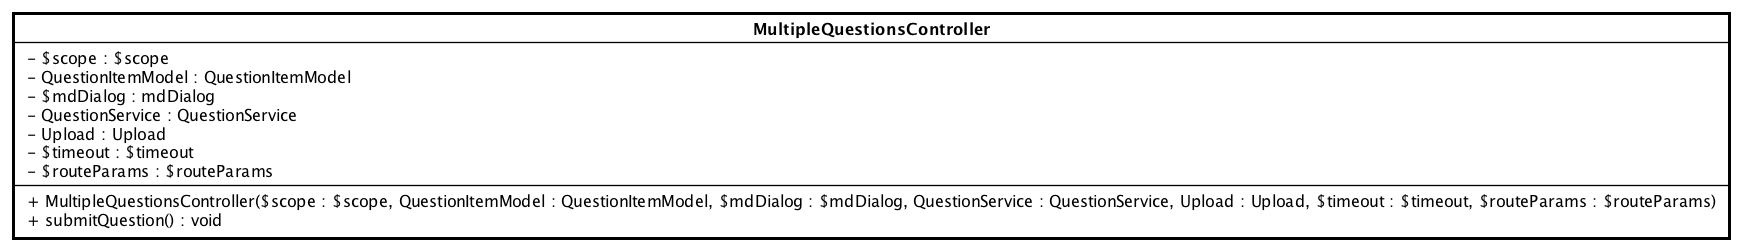
\includegraphics[scale=0.45]{UML/Classi/Front-End/QuizziPedia_Front-end_Controller_MultipleQuestionsController.png}
	\caption{QuizziPedia::Front-End::Controllers::MultipleChoiceQuestion}
\end{figure} \FloatBarrier
\begin{itemize}
	\item \textbf{Descrizione}: questa classe permette di gestire la creazione e la modifica di una domanda a risposta multipla;
	\item \textbf{Utilizzo}: fornisce le funzionalità per inserire una nuova domanda a risposta multipla nel database e per modificarne una esistente;
	\item \textbf{Relazione con altre classi}:
	\begin{itemize}
		\item \textit{IN} \texttt{MultipleQuestionsModelView}: ;
		\item \textit{IN} \texttt{QuestionService}: questa classe permette di ottenere domande esistenti e salvare nuove domande;
		\item \textit{IN} \texttt{QuestionItemModel}: è il modello (astratto) della domanda;
	\end{itemize}
	\item \textbf{Attributi}:
	\begin{itemize}
		\item \texttt{-} \texttt{\$scope: \$scope} \\
		Campo dati contenente un riferimento all’oggetto \$scope creato da \textit{Angular\ped{G}}, viene utilizzato come mezzo di comunicazione tra il controller e la view. Contiene gli oggetti che definiscono il model dell’applicazione;
		\item \texttt{-} \texttt{Question: QuestionItemModel} \\ Oggetto nel quale andremo a salvare la domanda dopo averla scaricata dal service (per poterla caricare nella view);
		\item \texttt{+} \texttt{\$cookie: \$cookie}: serve per recuperare l'id della domanda dalla pagina da cui arrivo;
		\item \texttt{-} \texttt{\$mdDialog: \$mdDialog} \\
		Campo dati contenente un riferimento al servizio della libreria \textit{Material for Angular\ped{G}} che permette di creare delle componenti a popup;
		\item \texttt{-} \texttt{QuestionService: QuestionService}: ;
	\end{itemize}
	\item \textbf{Metodi}:
	\begin{itemize}
		\item \texttt{+} \texttt{MultipleQuestionsController} \\ Costruttore della classe (controllerà anche se la domanda esiste (tramite cookie) e in caso la carica, altrimenti view con form vuota);
		\item \texttt{+} \texttt{submitQuestion}: raccoglie i dati dal modelview e li manda al service;
	\end{itemize}

\end{itemize}

\paragraph{QuizziPedia::Front-End::Controllers::ConnectionQuestionsController}
\begin{figure} [ht]
	\centering
	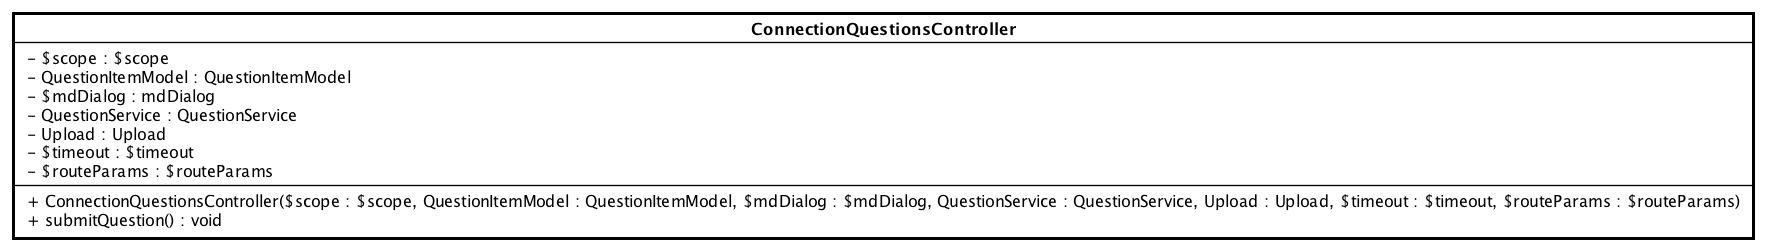
\includegraphics[scale=0.45]{UML/Classi/Front-End/QuizziPedia_Front-end_Controller_ConnectionQuestionsController.png}
	\caption{QuizziPedia::Front-End::Controllers::ConnectionQuestionsController}
\end{figure} \FloatBarrier
\begin{itemize}
	\item \textbf{Descrizione}: questa classe permette di gestire la creazione e la modifica di una domanda a collegamento;
	\item \textbf{Utilizzo}: fornisce le funzionalità per inserire una nuova domanda a collegamento nel database e per modificarne una esistente;
	\item \textbf{Relazione con altre classi}:
	\begin{itemize}
		\item \textit{IN} \texttt{ConnectionQuestionsModelView}: ;
		\item \textit{IN} \texttt{QuestionService}: questa classe permette di ottenere domande esistenti e salvare nuove domande;
		\item \textit{IN} \texttt{QuestionItemModel}: è il modello (astratto) della domanda;
	\end{itemize}
	\item \textbf{Attributi}:
	\begin{itemize}
		\item \texttt{-} \texttt{\$scope: \$scope} \\
		Campo dati contenente un riferimento all’oggetto \$scope creato da \textit{Angular\ped{G}}, viene utilizzato come mezzo di comunicazione tra il controller e la view. Contiene gli oggetti che definiscono il model dell’applicazione;
		\item \texttt{-} \texttt{Question: QuestionItemModel} \\ Oggetto nel quale andremo a salvare la domanda dopo averla scaricata dal service (per poterla caricare nella view);
		\item \texttt{+} \texttt{\$cookie: \$cookie}: serve per recuperare l'id della domanda dalla pagina da cui arrivo;
		\item \texttt{-} \texttt{\$mdDialog: \$mdDialog} \\
		Campo dati contenente un riferimento al servizio della libreria \textit{Material for Angular\ped{G}} che permette di creare delle componenti a popup;
		\item \texttt{-} \texttt{QuestionService: QuestionService}: ;
	\end{itemize}
	\item \textbf{Metodi}:
	\begin{itemize}
		\item \texttt{+} \texttt{ConnectionQuestionsController} \\ Costruttore della classe (controllerà anche se la domanda esiste (tramite cookie) e in caso la carica, altrimenti view con form vuota);
		\item \texttt{+} \texttt{submitQuestion}: raccoglie i dati dal modelview e li manda al service;
	\end{itemize}
\end{itemize}

\paragraph{QuizziPedia::Front-End::Controllers::ImagesSortingQuestionsController}
\begin{figure} [ht]
	\centering
	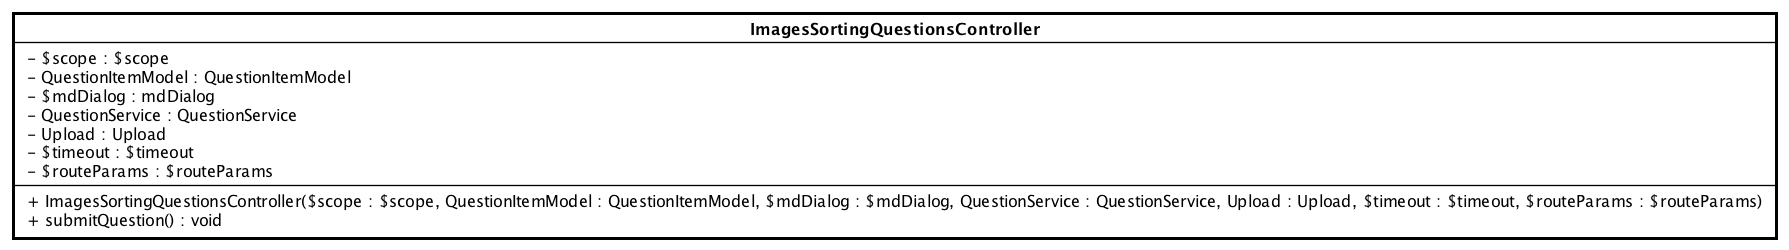
\includegraphics[scale=0.45]{UML/Classi/Front-End/QuizziPedia_Front-end_Controller_ImagesSortingQuestionsController.png}
	\caption{QuizziPedia::Front-End::Controllers::ImagesSortingQuestionsController}
\end{figure} \FloatBarrier
\begin{itemize}
	\item \textbf{Descrizione}: questa classe permette di gestire la creazione e la modifica di una domanda a ordinamento immagini;
	\item \textbf{Utilizzo}: fornisce le funzionalità per inserire una nuova domanda a ordinamento immagini nel database e per modificarne una esistente;
	\item \textbf{Relazione con altre classi}:
	\begin{itemize}
		\item \textit{IN} \texttt{ImageSortingQuestionsModelView}: ;
		\item \textit{IN} \texttt{QuestionService}: questa classe permette di ottenere domande esistenti e salvare nuove domande;
		\item \textit{IN} \texttt{QuestionItemModel}: è il modello (astratto) della domanda;
	\end{itemize}
	\item \textbf{Attributi}:
	\begin{itemize}
		\item \texttt{-} \texttt{\$scope: \$scope} \\
		Campo dati contenente un riferimento all’oggetto \$scope creato da \textit{Angular\ped{G}}, viene utilizzato come mezzo di comunicazione tra il controller e la view. Contiene gli oggetti che definiscono il model dell’applicazione;
		\item \texttt{-} \texttt{Question: QuestionItemModel} \\ Oggetto nel quale andremo a salvare la domanda dopo averla scaricata dal service (per poterla caricare nella view);
		\item \texttt{+} \texttt{\$cookie: \$cookie}: serve per recuperare l'id della domanda dalla pagina da cui arrivo;
		\item \texttt{-} \texttt{\$mdDialog: \$mdDialog} \\
		Campo dati contenente un riferimento al servizio della libreria \textit{Material for Angular\ped{G}} che permette di creare delle componenti a popup;
		\item \texttt{-} \texttt{QuestionService: QuestionService}: ;
	\end{itemize}
	\item \textbf{Metodi}:
	\begin{itemize}
		\item \texttt{+} \texttt{ImageSortingQuestionsController} \\ Costruttore della classe (controllerà anche se la domanda esiste (tramite cookie) e in caso la carica, altrimenti view con form vuota);
		\item \texttt{+} \texttt{submitQuestion}: raccoglie i dati dal modelview e li manda al service;
	\end{itemize}
\end{itemize}

\paragraph{QuizziPedia::Front-End::Controllers::StringsSortingQuestionsController}
\begin{figure} [ht]
	\centering
	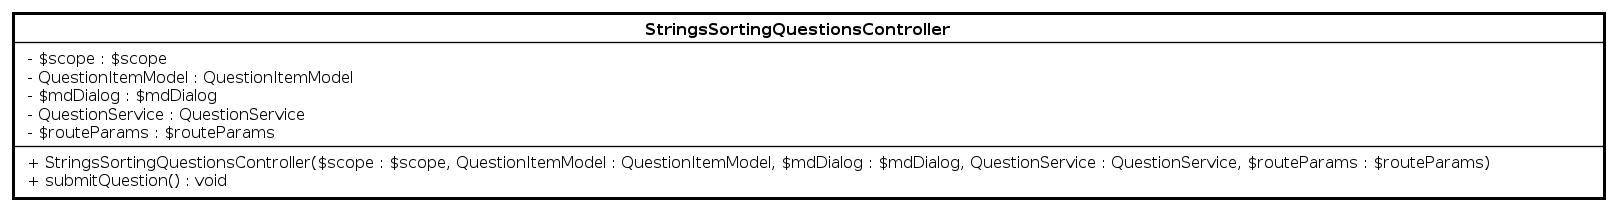
\includegraphics[scale=0.45]{UML/Classi/Front-End/QuizziPedia_Front-end_Controller_StringSortingQuestionsController.png}
	\caption{QuizziPedia::Front-End::Controllers::StringsSortingQuestionsController}
\end{figure} \FloatBarrier
\begin{itemize}
	\item \textbf{Descrizione}: questa classe permette di gestire la creazione e la modifica di una domanda a ordinamento di stringhe;
	\item \textbf{Utilizzo}: fornisce le funzionalità per inserire una nuova domanda a ordinamento di stringhe nel database e per modificarne una esistente;
	\item \textbf{Relazione con altre classi}:
	\begin{itemize}
		\item \textit{IN} \texttt{StringsSortingQuestionsModelView}: ;
		\item \textit{IN} \texttt{QuestionService}: questa classe permette di ottenere domande esistenti e salvare nuove domande;
		\item \textit{IN} \texttt{QuestionItemModel}: è il modello (astratto) della domanda;
	\end{itemize}
	\item \textbf{Attributi}:
	\begin{itemize}
		\item \texttt{-} \texttt{\$scope: \$scope} \\
		Campo dati contenente un riferimento all’oggetto \$scope creato da \textit{Angular\ped{G}}, viene utilizzato come mezzo di comunicazione tra il controller e la view. Contiene gli oggetti che definiscono il model dell’applicazione;
		\item \texttt{-} \texttt{Question: QuestionItemModel} \\ Oggetto nel quale andremo a salvare la domanda dopo averla scaricata dal service (per poterla caricare nella view);
		\item \texttt{+} \texttt{\$cookie: \$cookie}: serve per recuperare l'id della domanda dalla pagina da cui arrivo;
		\item \texttt{-} \texttt{\$mdDialog: \$mdDialog} \\
		Campo dati contenente un riferimento al servizio della libreria \textit{Material for Angular\ped{G}} che permette di creare delle componenti a popup;
		\item \texttt{-} \texttt{QuestionService: QuestionService}: ;
	\end{itemize}
	\item \textbf{Metodi}:
	\begin{itemize}
		\item \texttt{+} \texttt{StringsSortingQuestionsController} \\ Costruttore della classe (controllerà anche se la domanda esiste (tramite cookie) e in caso la carica, altrimenti view con form vuota);
		\item \texttt{+} \texttt{submitQuestion}: raccoglie i dati dal modelview e li manda al service;
	\end{itemize}
\end{itemize}

\paragraph{QuizziPedia::Front-End::Controllers::FillingQuestionsController}
\begin{figure} [ht]
	\centering
	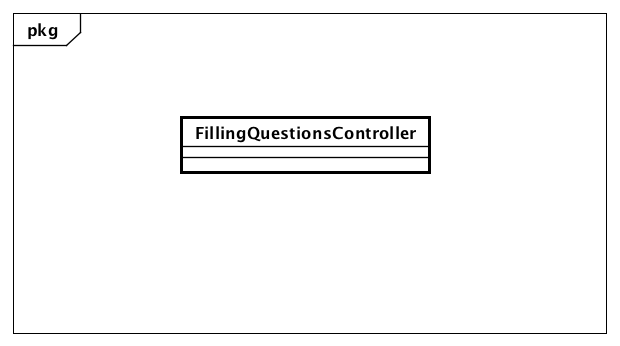
\includegraphics[scale=0.45]{UML/Classi/Front-End/QuizziPedia_Front-end_Controller_FillingQuestionsController.png}
	\caption{QuizziPedia::Front-End::Controllers::FillingQuestionsController}
\end{figure} \FloatBarrier
\begin{itemize}
	\item \textbf{Descrizione}: questa classe permette di gestire la creazione e la modifica di una domanda a riempimento di spazi;
	\item \textbf{Utilizzo}: fornisce le funzionalità per inserire una nuova domanda ariempimento di spazi nel database e per modificarne una esistente;
	\item \textbf{Relazione con altre classi}:
	\begin{itemize}
		\item \textit{IN} \texttt{FillingQuestionsModelView}: ;
		\item \textit{IN} \texttt{QuestionService}: questa classe permette di ottenere domande esistenti e salvare nuove domande;
		\item \textit{IN} \texttt{QuestionItemModel}: è il modello (astratto) della domanda;
	\end{itemize}
	\item \textbf{Attributi}:
	\begin{itemize}
		\item \texttt{-} \texttt{\$scope: \$scope} \\
		Campo dati contenente un riferimento all’oggetto \$scope creato da \textit{Angular\ped{G}}, viene utilizzato come mezzo di comunicazione tra il controller e la view. Contiene gli oggetti che definiscono il model dell’applicazione;
		\item \texttt{-} \texttt{Question: QuestionItemModel} \\ Oggetto nel quale andremo a salvare la domanda dopo averla scaricata dal service (per poterla caricare nella view);
		\item \texttt{+} \texttt{\$cookie: \$cookie}: serve per recuperare l'id della domanda dalla pagina da cui arrivo;
		\item \texttt{-} \texttt{\$mdDialog: \$mdDialog} \\
		Campo dati contenente un riferimento al servizio della libreria \textit{Material for Angular\ped{G}} che permette di creare delle componenti a popup;
		\item \texttt{-} \texttt{QuestionService: QuestionService}: ;
	\end{itemize}
	\item \textbf{Metodi}:
	\begin{itemize}
		\item \texttt{+} \texttt{FillingQuestionsController} \\ Costruttore della classe (controllerà anche se la domanda esiste (tramite cookie) e in caso la carica, altrimenti view con form vuota);
		\item \texttt{+} \texttt{submitQuestion}: raccoglie i dati dal modelview e li manda al service;
	\end{itemize}
\end{itemize}

\paragraph{QuizziPedia::Front-End::Controllers::ClickableAreaQuestionsController}
\begin{figure} [ht]
	\centering
	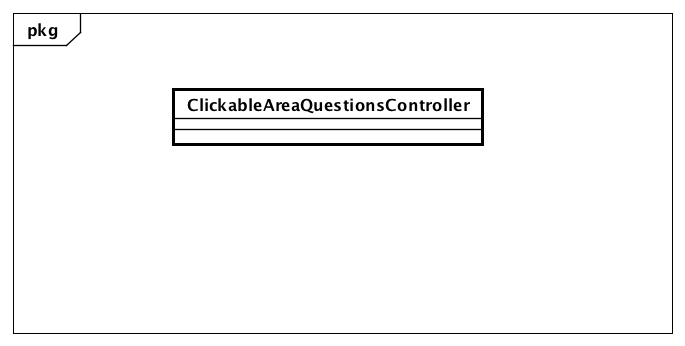
\includegraphics[scale=0.45]{UML/Classi/Front-End/QuizziPedia_Front-end_Controller_ClickableAreaQuestionsController.png}
	\caption{QuizziPedia::Front-End::Controllers::ClickableAreaQuestionsController}
\end{figure} \FloatBarrier
\begin{itemize}
	\item \textbf{Descrizione}: questa classe permette di gestire la creazione e la modifica di una domanda ad area cliccabile;
	\item \textbf{Utilizzo}: fornisce le funzionalità per inserire una nuova domanda ad area cliccabile nel database e per modificarne una esistente;
	\begin{itemize}
		\item \textit{IN} \texttt{ClickableAreaQuestionsModelView}: ;
		\item \textit{IN} \texttt{QuestionService}: questa classe permette di ottenere domande esistenti e salvare nuove domande;
		\item \textit{IN} \texttt{QuestionItemModel}: è il modello (astratto) della domanda;
	\end{itemize}
	\item \textbf{Attributi}:
	\begin{itemize}
		\item \texttt{-} \texttt{\$scope: \$scope} \\
		Campo dati contenente un riferimento all’oggetto \$scope creato da \textit{Angular\ped{G}}, viene utilizzato come mezzo di comunicazione tra il controller e la view. Contiene gli oggetti che definiscono il model dell’applicazione;
		\item \texttt{-} \texttt{Question: QuestionItemModel} \\ Oggetto nel quale andremo a salvare la domanda dopo averla scaricata dal service (per poterla caricare nella view);
		\item \texttt{+} \texttt{\$cookie: \$cookie}: serve per recuperare l'id della domanda dalla pagina da cui arrivo;
		\item \texttt{-} \texttt{\$mdDialog: \$mdDialog} \\
		Campo dati contenente un riferimento al servizio della libreria \textit{Material for Angular\ped{G}} che permette di creare delle componenti a popup;
		\item \texttt{-} \texttt{QuestionService: QuestionService}: ;
	\end{itemize}
	\item \textbf{Metodi}:
	\begin{itemize}
		\item \texttt{+} \texttt{ClickableAreaQuestionsController} \\ Costruttore della classe (controllerà anche se la domanda esiste (tramite cookie) e in caso la carica, altrimenti view con form vuota);
		\item \texttt{+} \texttt{submitQuestion}: raccoglie i dati dal modelview e li manda al service;
	\end{itemize}
\end{itemize}

\paragraph{QuizziPedia::Front-End::Controllers::EditorQMLController}
\begin{figure} [ht]
	\centering
	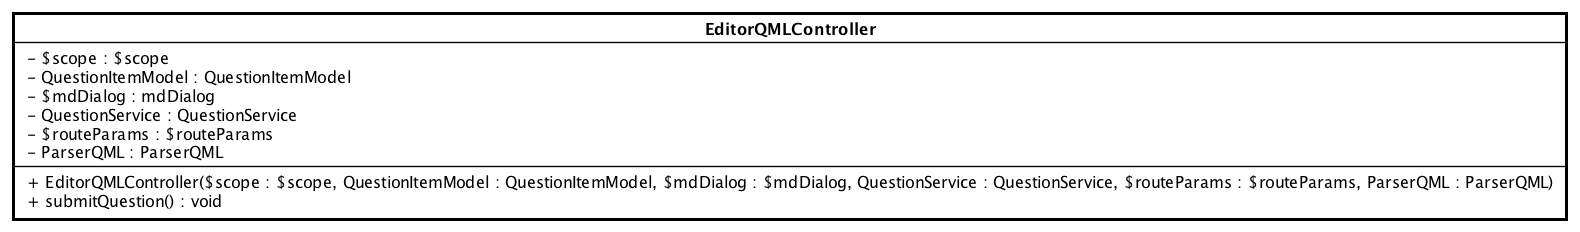
\includegraphics[scale=0.45]{UML/Classi/Front-End/QuizziPedia_Front-end_Controller_EditorQMLController.png}
	\caption{QuizziPedia::Front-End::Controllers::EditorQMLController}
\end{figure} \FloatBarrier
\begin{itemize}
	\item \textbf{Descrizione}: questa classe permette di gestire la creazione e la modifica di domande create tramite editor QML;
	\item \textbf{Utilizzo}: fornisce le funzionalità per creare e modificare una domanda tramite editor QML;
	\item \textbf{Relazione con altre classi}:
	\begin{itemize}
		\item \textit{IN} \texttt{EditorQMLView}: view contenente l'editor QML per la creazione di domande personalizzate; 
		\item \textit{OUT} \texttt{QuestionService}: questa classe permette di ottenere domande esistenti e salvare nuove domande;
	\end{itemize}
	\item \textbf{Attributi}:
	\begin{itemize}
		\item \texttt{-} \texttt{\$scope: \$scope} \\
		Campo dati contenente un riferimento all’oggetto \$scope creato da \textit{Angular\ped{G}}, viene utilizzato come mezzo di comunicazione tra il controller e la view. Contiene gli oggetti che definiscono il model dell’applicazione;
	\end{itemize}
	\item \textbf{Metodi}:
	\begin{itemize}
		\item 
	\end{itemize}
\end{itemize}

\paragraph{QuizziPedia::Front-End::Controllers::QuestionsManagementController}
\begin{figure} [ht]
	\centering
	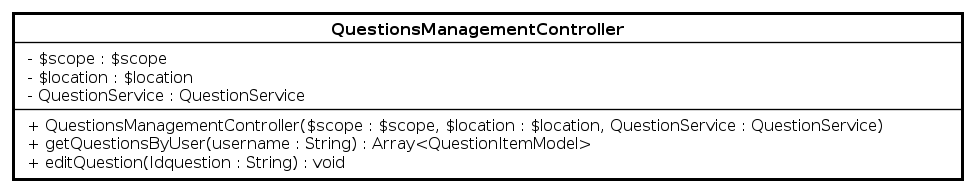
\includegraphics[scale=0.45]{UML/Classi/Front-End/QuizziPedia_Front-end_Controller_QuestionsManagementController.png}
	\caption{QuizziPedia::Front-End::Controllers::QuestionsManagementController}
\end{figure} \FloatBarrier
\begin{itemize}
	\item \textbf{Descrizione}: questa classe permette di gestire di ottenere le domande create dall'utente;
	\item \textbf{Utilizzo}: fornisce le funzionalità per richiedere al back-end le domande create dall'utente e mostrarle nella sua pagina personale; 
	\item \textbf{Relazione con altre classi}:
	\begin{itemize}
		\item \textit{IN} \texttt{QuestionsManagementModelView}: ; 
		\item \textit{IN} \texttt{QuestionService}: questa classe permette di ottenere domande esistenti e salvare nuove domande;
	\end{itemize}
	\item \textbf{Attributi}:
	\begin{itemize}
		\item \texttt{-} \texttt{\$scope: \$scope} \\
		Campo dati contenente un riferimento all’oggetto \$scope creato da \textit{Angular\ped{G}}, viene utilizzato come mezzo di comunicazione tra il controller e la view. Contiene gli oggetti che definiscono il model dell’applicazione;
		\item \texttt{-} \texttt{\$location: \$location} \\
		Campo dati contenente un riferimento al servizio creato da \textit{Angular\ped{G}} che permette di accedere alla barra degli indirizzi del \textit{browser\ped{G}}, i cambiamenti all’URL nella barra degli indirizzi si riflettono in questo oggetto e viceversa;
		\item \texttt{-} \texttt{QuestionService}
		\item \texttt{+} \texttt{\$cookie: \$cookie}: serve per passare l'id della domanda alla pagina che andrà a modificarla; 

	\end{itemize}
	\item \textbf{Metodi}:
	\begin{itemize}
		\item \texttt{+} \texttt{QuestionsManagementsController()} \\ Costruttore della classe;
		\item \texttt{-} \texttt{getQuestionsByUser(username: String)} \\ Prende le domande creare dall'utente e ne mostra un'anteprima;
		\item \texttt{+} \texttt{editQuestion()} \\ redirect a modifica domanda;
		
	\end{itemize}
\end{itemize}

\paragraph{QuizziPedia::Front-End::Controllers::TrainingController}
\begin{figure} [ht]
	\centering
	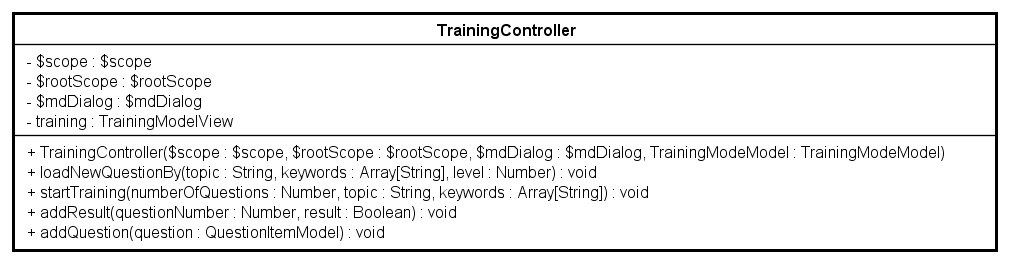
\includegraphics[scale=0.45]{UML/Classi/Front-End/QuizziPedia_Front-end_Controller_TrainingController.png}
	\caption{QuizziPedia::Front-End::Controllers::TrainingController}
\end{figure} \FloatBarrier
\begin{itemize}
	\item \textbf{Descrizione}: questa classe permette di gestire la modalità allenamento sottoponendo all'utente le giuste domande adatte al suo livello;
	\item \textbf{Utilizzo}: fornisce le funzionalità per recuperare le domande che siano in accordo con il livello dell'utente;
	\item \textbf{Relazione con altre classi}:
	\begin{itemize}
		\item \textit{IN} \texttt{TrainingModelView}: ;
		\item \textit{IN} \texttt{TrainingModeModel}: ?;
		\item \textit{IN} \texttt{TrainingSetUpTemplate}: rappresenta il componente grafico che permette all'utente di selezionare l'argomento e le parole chiave per iniziare un allenamento con queste caratteristiche. Viene gestito dinamicamente all'interno della view TrainingView attraverso il controller TrainingController;
		\item \textit{IN} \texttt{QuestionController}: ;
	\end{itemize}
	\item \textbf{Attributi}:
	\begin{itemize}
		\item \texttt{-} \texttt{\$scope: \$scope} \\
		Campo dati contenente un riferimento all’oggetto \$scope creato da \textit{Angular\ped{G}}, viene utilizzato come mezzo di comunicazione tra il controller e la view. Contiene gli oggetti che definiscono il model dell’applicazione;
		\item \texttt{-} \texttt{\$rootScope: \$rootScope} \\
		Campo dati contenente il riferimento all'oggetto globale \$rootScope creato da \textit{Angular\ped{G}}. Viene utilizzato per rendere accessibile a tutti i controller e a tutte le view l'oggetto \texttt{TrainingModeModel}. In questo caso viene utilizzato per inserire in \$rootScope l'oggetto di ritorno della chiamata a \texttt{getNextQuestion};
	\end{itemize}
	\item \textbf{Metodi}:
	\begin{itemize}
		\item \texttt{+} \texttt{TrainingController} \\ Metodo costruttore della classe;
		\item \texttt{-} \texttt{getNextQuestion} \\ Metodo che gestisce l'evento del click al pulsante "prossima domanda", fa una richiesta al QuestionController che ritornerà la domanda successiva.
	\end{itemize}
\end{itemize}

\paragraph{QuizziPedia::Front-End::Controllers::FillingQuestionnaireController}
\begin{figure} [ht]
	\centering
	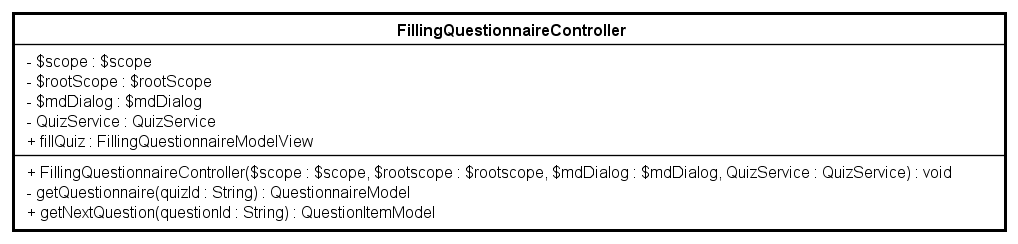
\includegraphics[scale=0.45]{UML/Classi/Front-End/QuizziPedia_Front-end_Controller_FillingQuestionnaireController.png}
	\caption{QuizziPedia::Front-End::Controllers::FillingQuestionnaireController}
\end{figure} \FloatBarrier
\begin{itemize}
	\item \textbf{Descrizione}: questa classe permette di gestire la compilazione del questionario;
	\item \textbf{Utilizzo}: fornisce le funzionalità per compilare un questionario e per gestire il cambio di domanda;
	\item \textbf{Relazione con altre classi}:
	\begin{itemize}
		\item \textit{IN} \texttt{FillingQuestionnaireModelView}: ;  
		\item \textit{IN} \texttt{InfoQuestionnaireTemplate}: rappresenta il componente grafico che permette all'utente di visualizzare le informazioni principali del questionario che si sta per svolgere. Viene gestito dinamicamente all'interno della view TrainingView attraverso il controller TrainingController;
		\item \textit{IN} \texttt{QuizService}: questa classe permette di ottenere i dati di un quiz tramite delle parole chiave inserite dall'utente nella barra di ricerca;
		\item \textit{IN} \texttt{QuestionnaireModel}: ;
		\item \textit{IN} \texttt{QuestionsController}: ; 
	\end{itemize}
	\item \textbf{Attributi}:
	\begin{itemize}
		\item \texttt{-} \texttt{\$scope: \$scope} \\
		Campo dati contenente un riferimento all’oggetto \$scope creato da \textit{Angular\ped{G}}, viene utilizzato come mezzo di comunicazione tra il controller e la view. Contiene gli oggetti che definiscono il model dell’applicazione;
		\item \texttt{-} \texttt{\$rootScope: \$rootScope} \\
		Campo dati contenente il riferimento all'oggetto globale \$rootScope creato da \textit{Angular\ped{G}}. Viene utilizzato per rendere accessibile a tutti i controller e a tutte le view l'oggetto \texttt{QuestionnaireModel}. In questo caso viene utilizzato per inserire in \$rootScope l'oggetto di ritorno della chiamata a \texttt{getNextQuestion} e la lista di puntatore ritornata dalla chiamata a \texttt{getQuestionsPreview};
	\end{itemize}
	\item \textbf{Metodi}:
	\begin{itemize}
		\item \texttt{+} \texttt{getQuestionsPreview}: \\ Metodo che permette di ottenere la lista di puntatori a tutte le domande del questionario;
		\item \texttt{+} \texttt{getNextQuestion}: \\ Metodo che ritorna la domanda successiva del quiz tramite chiamata a QuestionController;
	\end{itemize}
\end{itemize}

\paragraph{QuizziPedia::Front-End::Controllers::CreateQuestionnaireController}
\begin{figure} [ht]
	\centering
	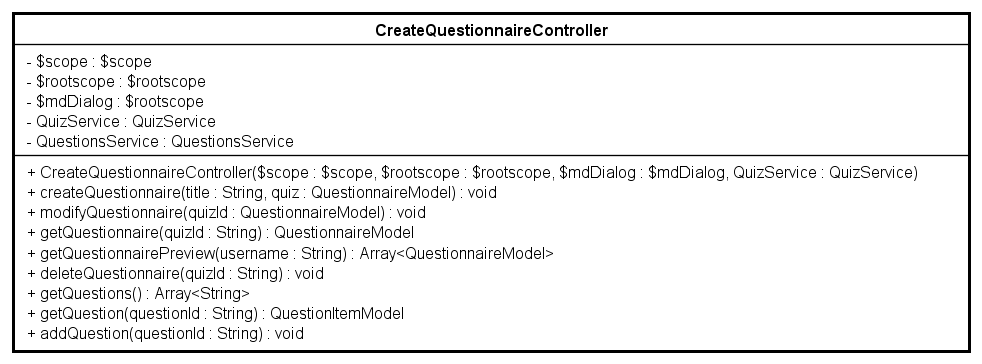
\includegraphics[scale=0.45]{UML/Classi/Front-End/QuizziPedia_Front-end_Controller_CreateQuestionnaireController.png}
	\caption{QuizziPedia::Front-End::Controllers::CreateQuestionnaireController}
\end{figure} \FloatBarrier
\begin{itemize}
	\item \textbf{Descrizione}: questa classe permette di gestire la creazione di un questionario;
	\item \textbf{Utilizzo}: fornisce tutte le funzionalità per la creazione di un nuovo questionario e per la modifica di uno esistente;
	\item \textbf{Relazione con altre classi}:
	\begin{itemize}
		\item \textit{IN} \texttt{CreateQuestionnaireModelView}: view per la creazione del questionario; 
		\item \textit{IN} \texttt{QuizService}: questa classe permette di ottenere i dati di un quiz tramite delle parole chiave inserite dall'utente nella barra di ricerca;
		\item \textit{IN} \texttt{TrainingModeModel}
	\end{itemize}
	\item \textbf{Attributi}:
	\begin{itemize}
		\item \texttt{-} \texttt{\$scope: \$scope} \\
		Campo dati contenente un riferimento all’oggetto \$scope creato da \textit{Angular\ped{G}}, viene utilizzato come mezzo di comunicazione tra il controller e la view. Contiene gli oggetti che definiscono il model dell’applicazione;
		\item \texttt{-} \texttt{\$rootScope: \$rootScope} \\
		Campo dati contenente il riferimento all'oggetto globale \$rootScope creato da \textit{Angular\ped{G}}. Viene utilizzato per rendere accessibile a tutti i controller e a tutte le view l'oggetto \texttt{TrainingModeModel}. In questo caso viene utilizzato per inserire in \$rootScope l'oggetto di ritorno della chiamata a \texttt{getQuestiontionnaire} e la lista dei questionari ottenuta dalla chiamata \texttt{getQuestionnairePreview};
		\item \texttt{-} \texttt{QuizService}: ;
	\end{itemize}
	\item \textbf{Metodi}:
	\begin{itemize}
		\item \texttt{+} \texttt{CreateQuestionnaireController}: \\ Metodo costruttore della classe
		\item \texttt{+} \texttt{createQuestionnaire(passerò l'oggetto questionario in trainingModeModel)}: ;
		\item \texttt{+} \texttt{modifyQuestionnaire(passerò l'oggetto modificato)}: ;
		\item \texttt{+} \texttt{getQuestionnaire(id questionario che voglio modificare)}: ;
		\item \texttt{+} \texttt{getQuestionnairePreview(username: String)}: serve per ottenere la lista di tutti i questionari di un utente;
	\end{itemize}
\end{itemize}

\paragraph{QuizziPedia::Front-End::Controllers::RegistrationManagementController}
\begin{figure} [ht]
	\centering
	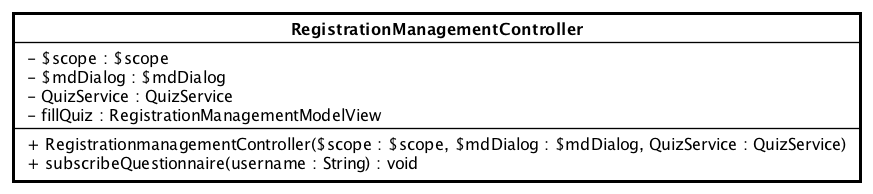
\includegraphics[scale=0.45]{UML/Classi/Front-End/QuizziPedia_Front-end_Controller_RegistrationManagementController.png}
	\caption{QuizziPedia::Front-End::Controllers::RegistrationManagementController}
\end{figure} \FloatBarrier
\begin{itemize}
	\item \textbf{Descrizione}: questa classe permette di gestire le iscrizione degli utenti ai questionari;
	\item \textbf{Utilizzo}: fornisce le funzionalità di iscrizione ad un questionario;
	\item \textbf{Relazione con altre classi}:
	\begin{itemize}
		\item \textit{IN} \texttt{RegistratioManagementView}: view per la gestione degli utenti iscritti a un proprio questionario; 
		\item \textit{OUT} \texttt{QuizService}: questa classe permette di ottenere i dati di un quiz tramite delle parole chiave inserite dall'utente nella barra di ricerca;
	\end{itemize}
	\item \textbf{Attributi}:
	\begin{itemize}
		\item \texttt{-} \texttt{\$scope: \$scope} \\
		Campo dati contenente un riferimento all’oggetto \$scope creato da \textit{Angular\ped{G}}, viene utilizzato come mezzo di comunicazione tra il controller e la view. Contiene gli oggetti che definiscono il model dell’applicazione;
	\end{itemize}
	\item \textbf{Metodi}:
	\begin{itemize}
		\item 
	\end{itemize}
\end{itemize}

\paragraph{QuizziPedia::Front-End::Controllers::ResultsController}
\begin{figure} [ht]
	\centering
	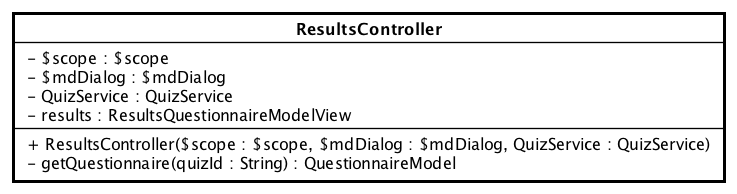
\includegraphics[scale=0.45]{UML/Classi/Front-End/QuizziPedia_Front-end_Controller_ResultsController.png}
	\caption{QuizziPedia::Front-End::Controllers::ResultsController}
\end{figure} \FloatBarrier
\begin{itemize}
	\item \textbf{Descrizione}: questa classe permette di gestire i risultati della ricerca effettuata dall'utente;
	\item \textbf{Utilizzo}: fornisce le funzionalità per recuperare i dati dal back-end e mostrarli all'utente nella view;
	\item \textbf{Relazione con altre classi}:
	\begin{itemize}
		\item \textit{IN} \texttt{ResultsQuestionnaireView}: view contenente i risultati della ricerca effettuata, sia gli utenti che i questionari; 
		\item \textit{OUT} \texttt{QuizService}: questa classe permette di ottenere i dati di un quiz tramite delle parole chiave inserite dall'utente nella barra di ricerca;
	\end{itemize}
	\item \textbf{Attributi}:
	\begin{itemize}
		\item \texttt{-} \texttt{\$scope: \$scope} \\
		Campo dati contenente un riferimento all’oggetto \$scope creato da \textit{Angular\ped{G}}, viene utilizzato come mezzo di comunicazione tra il controller e la view. Contiene gli oggetti che definiscono il model dell’applicazione;
	\end{itemize}
	\item \textbf{Metodi}:
	\begin{itemize}
		\item 
	\end{itemize}
\end{itemize}

\paragraph{QuizziPedia::Front-End::Controllers::QuestionnaireManagementController}
\begin{figure} [ht]
	\centering
	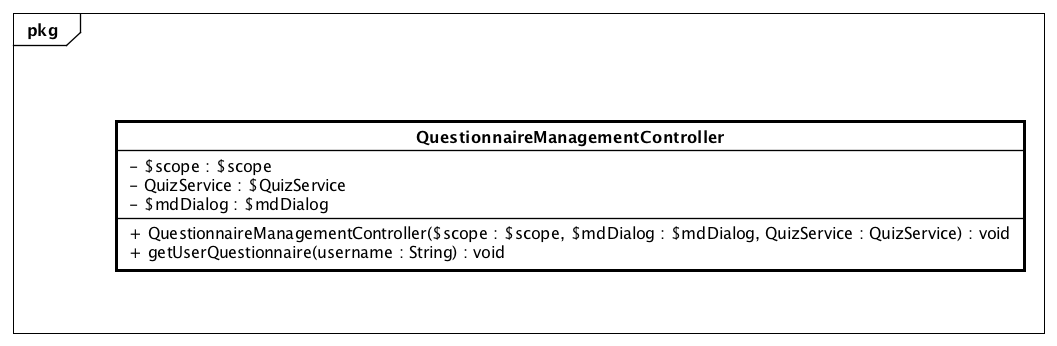
\includegraphics[scale=0.45]{UML/Classi/Front-End/QuizziPedia_Front-end_Controller_QuestionnaireManagementController.png}
	\caption{QuizziPedia::Front-End::Controllers::QuestionnaireManagementController}
\end{figure} \FloatBarrier
\begin{itemize}
	\item \textbf{Descrizione}: questa classe permette di gestire tutti i questionari creati da un utente; 
	\item \textbf{Utilizzo}: fornisce le funzionalità per recuperare dal back-end tutti i questionari creati da un utente;
	\item \textbf{Relazione con altre classi}:
	\begin{itemize}
		\item \textit{IN} \texttt{QuestionnaireManagementeView}: view principale per la gestione dei questionari;
		\item \textit{OUT} \texttt{QuizService}: questa classe permette di ottenere i dati di un quiz tramite delle parole chiave inserite dall'utente nella barra di ricerca;
	\end{itemize}
	\item \textbf{Attributi}:
	\begin{itemize}
		\item \texttt{-} \texttt{\$scope: \$scope} \\
		Campo dati contenente un riferimento all’oggetto \$scope creato da \textit{Angular\ped{G}}, viene utilizzato come mezzo di comunicazione tra il controller e la view. Contiene gli oggetti che definiscono il model dell’applicazione;
	\end{itemize}
	\item \textbf{Metodi}:
	\begin{itemize}
		\item 
	\end{itemize}
\end{itemize}

\paragraph{QuizziPedia::Front-End::Controllers::MenuBarController}
\begin{figure} [ht]
	\centering
	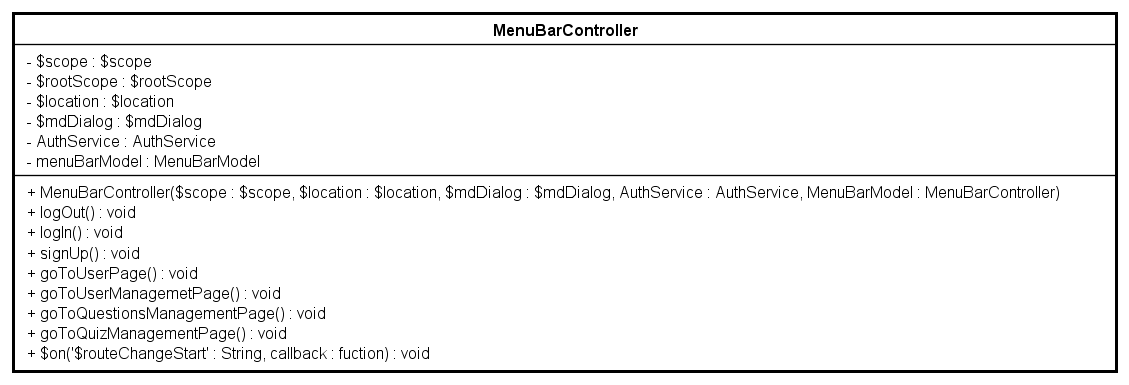
\includegraphics[scale=0.45]{UML/Classi/Front-End/QuizziPedia_Front-end_Controller_MenuBarController.png}
	\caption{QuizziPedia::Front-End::Controllers::MenuBarController}
\end{figure} \FloatBarrier
\begin{itemize}
	\item \textbf{Descrizione}: questa classe permette di gestire il menù fisso per ogni pagina;
	\item \textbf{Utilizzo}: fornisce le funzionalità per aggiornare, a seconda della pagina, il contenuto del menù;
	\item \textbf{Relazione con altre classi}:
	\begin{itemize}
		\item \textit{IN} \texttt{MenuBarDirective}: rappresenta il menù, presente in ogni pagina dell'applicazione, generato in base agli oggetti passati nello \$scope isolato. Fornisce un pulsante per ogni oggetto ricevuto come parametro, ogni pulsante viene rappresentato con un’icona e con un testo. Al click di un pulsante viene invocata la funzione ad esso associata;  
	\end{itemize}
	\item \textbf{Attributi}:
	\begin{itemize}
		\item \texttt{-} \texttt{\$scope: \$scope} \\
		Campo dati contenente un riferimento all’oggetto \$scope creato da \textit{Angular\ped{G}}, viene utilizzato come mezzo di comunicazione tra il controller e la view. Contiene gli oggetti che definiscono il model dell’applicazione;
	\end{itemize}
	\item \textbf{Metodi}:
	\begin{itemize}
		\item 
	\end{itemize}
\end{itemize}

\paragraph{QuizziPedia::Front-End::Controllers::FooterController}
\begin{figure} [ht]
	\centering
	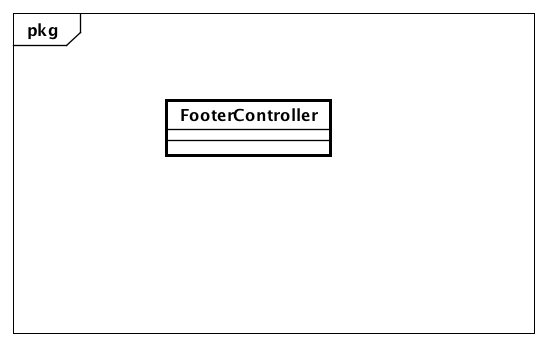
\includegraphics[scale=0.45]{UML/Classi/Front-End/QuizziPedia_Front-end_Controller_FooterController.png}
	\caption{QuizziPedia::Front-End::Controllers::FooterController}
\end{figure} \FloatBarrier
\begin{itemize}
	\item \textbf{Descrizione}: questa classe permette di gestire il footer dell'applicazione;
	\item \textbf{Utilizzo}: fornisce le funzionalità per recuperare le informazioni da mostrare nel footer;
	\item \textbf{Relazione con altre classi}:
	\begin{itemize}
		\item \textit{IN} \texttt{FooterDirective}: directive che mostra il footer dell'applicazione che sarà presente in ogni pagina;  
	\end{itemize}
	\item \textbf{Attributi}:
	\begin{itemize}
		\item \texttt{-} \texttt{\$scope: \$scope} \\
		Campo dati contenente un riferimento all’oggetto \$scope creato da \textit{Angular\ped{G}}, viene utilizzato come mezzo di comunicazione tra il controller e la view. Contiene gli oggetti che definiscono il model dell’applicazione;
	\end{itemize}
	\item \textbf{Metodi}:
	\begin{itemize}
		\item 
	\end{itemize}
\end{itemize}

\paragraph{QuizziPedia::Front-End::Controllers::QuestionnaireDetailsController}
\begin{figure} [ht]
	\centering
	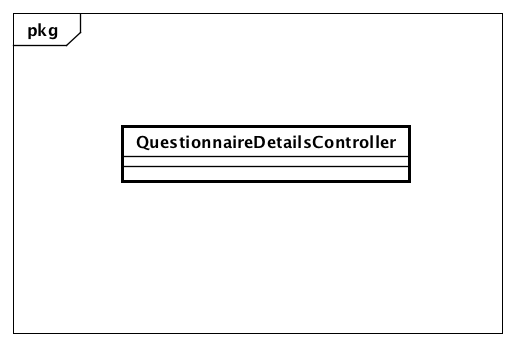
\includegraphics[scale=0.45]{UML/Classi/Front-End/QuizziPedia_Front-end_Controller_QuestionnaireDetailsController.png}
	\caption{QuizziPedia::Front-End::Controllers::QuestionnaireDetailsController}
\end{figure} \FloatBarrier
\begin{itemize}
	\item \textbf{Descrizione}: questa classe permette di gestire i dettagli di un questionario; 
	\item \textbf{Utilizzo}: fornisce le funzionalità per recuperare dal back-end i dettagli di un questionario creato da un utente al fine di poterli visualizzare nel suo profilo;
	\item \textbf{Relazione con altre classi}:
	\begin{itemize}
		\item \textit{IN} \texttt{QuestionnaireDetailsModelView}: ;
		\item \textit{IN} \texttt{QuizService}: questa classe permette di ottenere i dati di un quiz tramite delle parole chiave inserite dall'utente nella barra di ricerca;
		\item \textit{} \texttt{QuestionnaireModel}: ;
	\end{itemize}
	\item \textbf{Attributi}:
	\begin{itemize}
		\item \texttt{-} \texttt{\$scope: \$scope} \\
		Campo dati contenente un riferimento all’oggetto \$scope creato da \textit{Angular\ped{G}}, viene utilizzato come mezzo di comunicazione tra il controller e la view. Contiene gli oggetti che definiscono il model dell’applicazione;
		\item \texttt{-} \texttt{\$rootScope: \$rootScope} \\
		Campo dati contenente il riferimento all'oggetto globale \$rootScope creato da \textit{Angular\ped{G}}. Viene utilizzato per rendere accessibile a tutti i controller e a tutte le view l'oggetto \texttt{QuestionnaireModel}. In questo caso viene utilizzato per inserire in \$rootScope l'oggetto di ritorno della chiamata a \texttt{getQuestionnaireDetails} del service \texttt{QuizService};

	\end{itemize}
	\item \textbf{Metodi}:
	\begin{itemize}
		\item \texttt{+} \texttt{QuestionnaireDetailsController}: \\ Metodo costruttore della classe;
		\item \texttt{-} \texttt{getQuestionnaireDetails(username: String)}: \\ Metodo che richiede al service i dettagli dei questionari
	\end{itemize}
\end{itemize}

\paragraph{QuizziPedia::Front-End::Controllers::UserDetailsController}
\begin{figure} [ht]
	\centering
	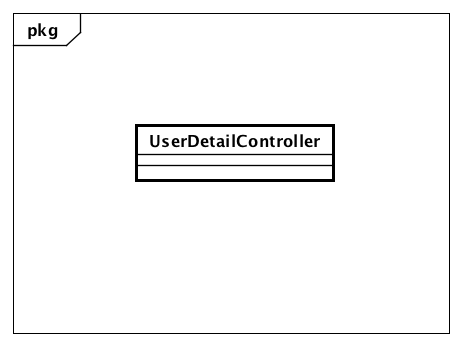
\includegraphics[scale=0.45]{UML/Classi/Front-End/QuizziPedia_Front-end_Controller_UserDetailController.png}
	\caption{QuizziPedia::Front-End::Controllers::UserDetailController}
\end{figure} \FloatBarrier
\begin{itemize}
	\item \textbf{Descrizione}: questa classe permette di ottenere i dati di un utente;
	\item \textbf{Utilizzo}: fornisce le funzionalità per ottenere i dati di un utente per poterle mostrare nella view;
	\item \textbf{Relazione con altre classi}:
	\begin{itemize}
		\item \textit{IN} \texttt{UserDetailsModelView}: directive che permette di visualizzare i dati di un utente; 
		\item \textit{IN} \texttt{UserDetailsService}: questa classe permette di ottenere i dati dell'utente;
		\item \textit{IN} \texttt{UserDetailsModel}: 
	\end{itemize}
	\item \textbf{Attributi}:
	\begin{itemize}
		\item \texttt{-} \texttt{\$scope: \$scope} \\
		Campo dati contenente un riferimento all’oggetto \$scope creato da \textit{Angular\ped{G}}, viene utilizzato come mezzo di comunicazione tra il controller e la view. Contiene gli oggetti che definiscono il model dell’applicazione;
		\item \texttt{-} \texttt{\$rootScope: \$rootScope} \\
		Campo dati contenente il riferimento all'oggetto globale \$rootScope creato da \textit{Angular\ped{G}}. Viene utilizzato per rendere accessibile a tutti i controller e a tutte le view l'oggetto \texttt{UserDetailsModel}. In questo caso viene utilizzato per inserire in \$rootScope l'oggetto di ritorno della chiamata a \texttt{getUserDetails} del service \texttt{UserDetailsService};
		\item \texttt{-} \texttt{userDetailsService}: parametro permette di ottenere i dati dell'utente;
	\end{itemize}	
	\begin{itemize}
		\item \textbf{Metodi}:
		\item \texttt{+} \texttt{UserDetailsController()} \\ Metodo costruttore della classe;
		\item \texttt{-} \texttt{getUserDetails(username: String)} \\ Metodo che permette di ottenere i dati con una chiamata a UserDetailsService;
	\end{itemize}
\end{itemize}

\paragraph{QuizziPedia::Front-End::Controllers::QuestionsController}
\begin{figure} [ht]
	\centering
	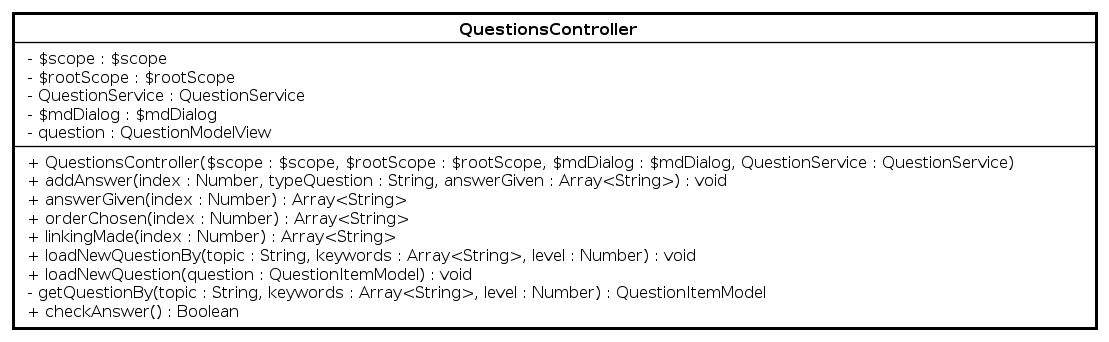
\includegraphics[scale=0.45]{UML/Classi/Front-End/QuizziPedia_Front-end_Controller_QuestionsController.png}
	\caption{QuizziPedia::Front-End::Controllers::QuestionsController}
\end{figure} \FloatBarrier
\begin{itemize}
	\item \textbf{Descrizione}: questa classe permette di gestire il recupero delle domande per poterle stampare nella modalità allenamento;
	\item \textbf{Utilizzo}: fornisce le funzionalità per il recupero delle domande esistenti nel database al fine di mostrarle durante la modalità allenamento nell'apposito template;
	\item \textbf{Relazione con altre classi}:
	\begin{itemize}
		\item \textit{IN} \texttt{HeaderTextQuestionTemplate}: rappresenta il componente grafico che presenta all'utente il testo della domanda, l'argomento e le parole chiave. Viene gestito dinamicamente all'interno della view TrainingView attraverso il controller TrainingController; 
		\item \textit{IN} \texttt{TrueFalseAnswerTemplate}: rappresenta il componente grafico che permette all'utente di visualizzare la domanda vero e falso. Viene gestito dinamicamente all'interno della view TrainingView attraverso il controller TrainingController; 
		\item \textit{IN} \texttt{MultipleChoiceAnswerTemplate}: rappresenta il componente grafico che permette all'utente di visualizzare la domanda a risposta multipla. Viene gestito dinamicamente all'interno della view TrainingView attraverso il controller TrainingController; 
		\item \textit{IN} \texttt{LinkingAnswerTemplate}: rappresenta il componente grafico che permette all'utente di visualizzare la domanda di collegamento. Viene gestito dinamicamente all'interno della view TrainingView attraverso il controller TrainingController; 
		\item \textit{IN} \texttt{SortImagesAnswerTemplate}: rappresenta il componente grafico che permette all'utente di visualizzare la domanda ad ordinamento di immagini. Viene gestito dinamicamente all'interno della view TrainingView attraverso il controller TrainingController; 
		\item \textit{IN} \texttt{SortTextAnswerTemplate}: rappresenta il componente grafico che permette all'utente di visualizzare la domanda ad ordinamento di stringhe. Viene gestito dinamicamente all'interno della view TrainingView attraverso il controller TrainingController; 
		\item \textit{IN} \texttt{EmptySpaceAnswerTemplate}: rappresenta il componente grafico che permette all'utente di visualizzare l'esercizio a riempimento di spazi vuoti. Viene gestito dinamicamente all'interno della view TrainingView attraverso il controller TrainingController; 
		\item \textit{IN} \texttt{ClickableAnswerTemplate}: rappresenta il componente grafico che permette all'utente di visualizzare la domanda ad area cliccabile nell'immagine. Viene gestito dinamicamente all'interno della view TrainingView attraverso il controller TrainingController;  
		\item \textit{IN} \texttt{QuestionServices}: questa classe permette di ottenere domande esistenti e salvare nuove domande;
		\item \textit{IN} \texttt{QuestionItemModel}: ;
		\item \textit{OUT} \texttt{FillingQuestionnaireController}: ;
		
	\end{itemize}
	\item \textbf{Attributi}:
	\begin{itemize}
		\item \texttt{-} \texttt{\$scope: \$scope} \\
		Campo dati contenente un riferimento all’oggetto \$scope creato da \textit{Angular\ped{G}}, viene utilizzato come mezzo di comunicazione tra il controller e la view. Contiene gli oggetti che definiscono il model dell’applicazione;
		\item \texttt{-} \texttt{\$rootScope: \$rootScope} \\
		Campo dati contenente il riferimento all'oggetto globale \$rootScope creato da \textit{Angular\ped{G}}. Viene utilizzato per rendere accessibile a tutti i controller e a tutte le view l'oggetto \texttt{QuestionItemModel}. In questo caso viene utilizzato per inserire in \$rootScope l'oggetto di ritorno della chiamata a \texttt{getQuestion} del service \texttt{QuestionService};
		\item \texttt{-} \texttt{QuestionService}: ;
	\end{itemize}
	\item \textbf{Metodi}:
	\begin{itemize}
		\item \texttt{+} \texttt{QuestionsController}: \\ Metodo costruttore della classe
		\item \texttt{+} \texttt{getQuestion}: \\ Metodo che richiede al back-end una domanda;
	\end{itemize}
\end{itemize}

\paragraph{QuizziPedia::Front-End::Controllers::TopicKeywordsController}
\begin{figure} [ht]
	\centering
	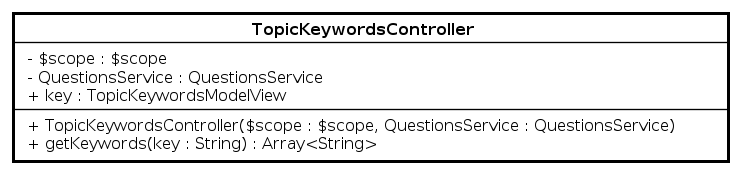
\includegraphics[scale=0.45]{UML/Classi/Front-End/QuizziPedia_Front-end_Controller_TopicKeywordsController.png}
	\caption{QuizziPedia::Front-End::Controllers::TopicKeywordsController}
\end{figure} \FloatBarrier
\begin{itemize}
	\item \textbf{Descrizione}: questa classe permette di gestire il recupero delle parole chiave di un questionario;
	\item \textbf{Utilizzo}: fornisce le funzionalità per il recupero delle parole chiave durante la creazione di un questionario;
	\item \textbf{Relazione con altre classi}:
	\begin{itemize}
		\item \textit{IN} \texttt{TopicKeywordsDirective}: directive che permette di gestire l'inserimento di keywords al momento della creazione della domanda; 
		\item \textit{IN} \texttt{QuestionsService}: questa classe permette di ottenere domande esistenti e salvare nuove domande; 
	\end{itemize}
	\item \textbf{Attributi}:
	\begin{itemize}
		\item \texttt{-} \texttt{\$scope: \$scope} \\
		Campo dati contenente un riferimento all’oggetto \$scope creato da \textit{Angular\ped{G}}, viene utilizzato come mezzo di comunicazione tra il controller e la view. Contiene gli oggetti che definiscono il model dell’applicazione;
	\end{itemize}
	\item \textbf{Metodi}:
	\begin{itemize}
		\item 
	\end{itemize}
\end{itemize}

\paragraph{QuizziPedia::Front-End::Controllers::QuestionnaireQuestionsManagementController}
\begin{figure} [ht]
	\centering
	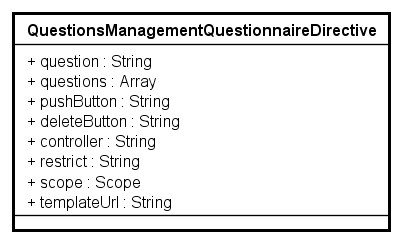
\includegraphics[scale=0.45]{UML/Classi/Front-End/QuizziPedia_Front-end_Controller_QuestionnaireQuestionsManagementController.png}
	\caption{QuizziPedia::Front-End::Controllers::QuestionnaireQuestionsManagementController}
\end{figure} \FloatBarrier
\begin{itemize}
	\item \textbf{Descrizione}: questa classe permette di gestire il recupero delle domande per il questionario;
	\item \textbf{Utilizzo}: fornisce le funzionalità per il recupero delle domande dal back-end e le rende disponibili per poter popolare le view;
	\item \textbf{Relazione con altre classi}:
	\begin{itemize}
		\item \textit{IN} \texttt{QuestionnaireQuestionsManagementDirective}: rappresenta il componente grafico che permette all'utente di:
		\begin{itemize}
			\item Effettuare delle ricerche sul database di domande;
			\item Selezionare le domande da inserire nel questionario;
			\item Mostrare le domande già inserite e permettere all'utente di eliminarle da tale lista.
		\end{itemize}
		Questo componente si presta sia per la creazione che per la modifica di un questionario;
		\item \textit{IN} \texttt{QuestionsService}: questa classe permette di ottenere domande esistenti e salvare nuove domande;
	\end{itemize}
	\item \textbf{Attributi}:
	\begin{itemize}
		\item \texttt{-} \texttt{\$scope: \$scope} \\
		Campo dati contenente un riferimento all’oggetto \$scope creato da \textit{Angular\ped{G}}, viene utilizzato come mezzo di comunicazione tra il controller e la view. Contiene gli oggetti che definiscono il model dell’applicazione;
	\end{itemize}
	\item \textbf{Metodi}:
	\begin{itemize}
		\item 
	\end{itemize}
\end{itemize}

\paragraph{QuizziPedia::Front-End::Controllers::InputToListController}
\begin{figure} [ht]
	\centering
	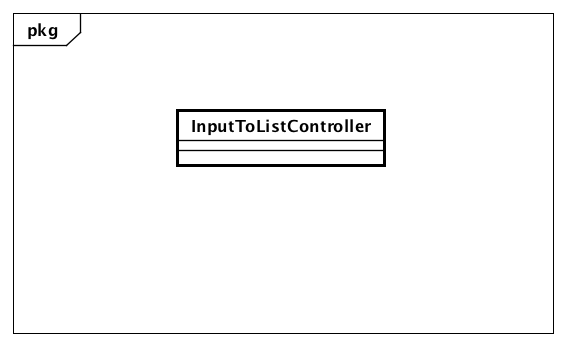
\includegraphics[scale=0.45]{UML/Classi/Front-End/QuizziPedia_Front-end_Controller_InputToListController.png}
	\caption{QuizziPedia::Front-End::Controllers::InputToListController}
\end{figure} \FloatBarrier
\begin{itemize}
	\item \textbf{Descrizione}: questa classe permette di gestire l'inserimento di una lista di risposte durante la creazione di una domanda;
	\item \textbf{Utilizzo}: fornisce le funzionalità per confermare porzioni di domanda durante la creazione;
	\item \textbf{Relazione con altre classi}:
	\begin{itemize}
		\item \textit{IN} \texttt{ConnectionQuestionsView}: view contenente i campi per creare una domanda a collegamento;
		\item \textit{IN} \texttt{StringsSortingQuestionsView}: view contenente i campi per creare una domanda a ordinamento stringhe; 
		\item \textit{IN} \texttt{ImagesSortingQuestionsView}: view contenente i campi per creare una domanda a ordinamento immmagini;
	\end{itemize}
	\item \textbf{Attributi}:
	\begin{itemize}
		\item \texttt{-} \texttt{\$scope: \$scope} \\
		Campo dati contenente un riferimento all’oggetto \$scope creato da \textit{Angular\ped{G}}, viene utilizzato come mezzo di comunicazione tra il controller e la view. Contiene gli oggetti che definiscono il model dell’applicazione;
	\end{itemize}
	\item \textbf{Metodi}:
	\begin{itemize}
		\item 
	\end{itemize}
\end{itemize}

\paragraph{QuizziPedia::Front-End::Controllers::NewQuestionsButtonController}
\begin{figure} [ht]
	\centering
	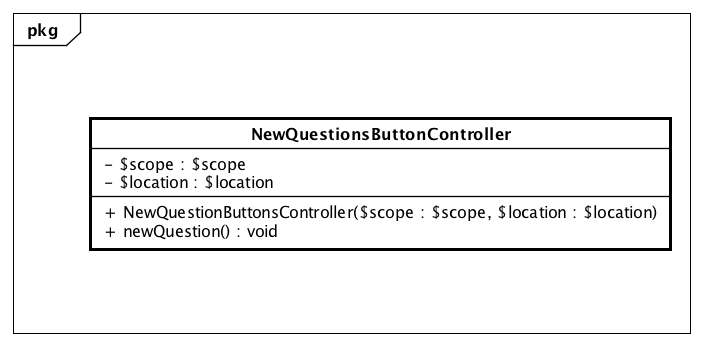
\includegraphics[scale=0.45]{UML/Classi/Front-End/QuizziPedia_Front-end_Controller_NewQuestionsButtonController.png}
	\caption{QuizziPedia::Front-End::Controllers::NewQuestionButtonController}
\end{figure} \FloatBarrier
\begin{itemize}
	\item \textbf{Descrizione}: questa classe permette di effettuare il redirect alla pagina di creazione nuova domanda;
	\item \textbf{Utilizzo}: effettua il redirect alla pagina di creazione nuova domanda quando l'utente seleziona l'apposito link;
	\item \textbf{Relazione con altre classi}:
	\begin{itemize}
		\item \textit{IN} \texttt{NewQuestionButtonsModelView}: ; 
	\end{itemize}
	\item \textbf{Attributi}:
	\begin{itemize}
		\item \texttt{-} \texttt{\$scope: \$scope} \\
		Campo dati contenente un riferimento all’oggetto \$scope creato da \textit{Angular\ped{G}}, viene utilizzato come mezzo di comunicazione tra il controller e la view. Contiene gli oggetti che definiscono il model dell’applicazione;
		\item \texttt{-} \texttt{\$location: \$location} \\
		Campo dati contenente un riferimento al servizio creato da \textit{Angular\ped{G}} che permette di accedere alla barra degli indirizzi del \textit{browser\ped{G}}, i cambiamenti all’URL nella barra degli indirizzi si riflettono in questo oggetto e viceversa;
	\end{itemize}
	\item \textbf{Metodi}:
	\begin{itemize}
		\item \texttt{+} \texttt{NewQuestionButtonsController()} \\ Metodo costruttore della classe;
		\item \texttt{+} \texttt{newQuestion()} \\ redirect a creazione domanda;
	\end{itemize}
\end{itemize}

\paragraph{QuizziPedia::Front-End::Controllers::StatisticsController}
\begin{figure} [ht]
	\centering
	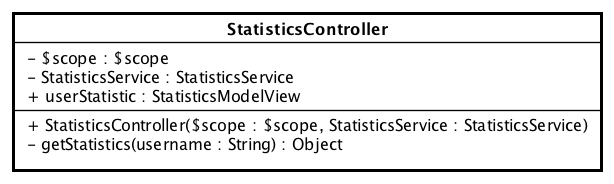
\includegraphics[scale=0.45]{UML/Classi/Front-End/QuizziPedia_Front-end_Controller_StatisticsController.png}
	\caption{QuizziPedia::Front-End::Controllers::StatisticsController}
\end{figure} \FloatBarrier
\begin{itemize}
	\item \textbf{Descrizione}: questa classe permette di le statistiche di un utente;
	\item \textbf{Utilizzo}: fornisce le funzionalità per ottenere le statistiche di un utente per poterle mostrare nella view;
	\item \textbf{Relazione con altre classi}:
	\begin{itemize}
		\item \textit{IN} \texttt{StatisticsModelView}: directive che permette di visualizzare le statistiche di un utente; 
		\item \textit{IN} \texttt{StatisticsService}: questa classe permette di ottenere le statistiche dell'utente;
		\item \textit{IN} \texttt{UserDetailsModel}: 
	\end{itemize}
	\item \textbf{Attributi}:
	\begin{itemize}
		\item \texttt{-} \texttt{\$scope: \$scope} \\
		Campo dati contenente un riferimento all’oggetto \$scope creato da \textit{Angular\ped{G}}, viene utilizzato come mezzo di comunicazione tra il controller e la view. Contiene gli oggetti che definiscono il model dell’applicazione;
		\item \texttt{-} \texttt{\$rootScope: \$rootScope} \\
		Campo dati contenente il riferimento all'oggetto globale \$rootScope creato da \textit{Angular\ped{G}}. Viene utilizzato per rendere accessibile a tutti i controller e a tutte le view l'oggetto \texttt{UserDetailsModel}. In questo caso viene utilizzato per inserire in \$rootScope l'oggetto di ritorno della chiamata a \texttt{getStatistics} del service \texttt{StatisticsService};
		\item \texttt{-} \texttt{StatisticsService}: parametro permette di ottenere le statistiche dell'utente;
	\end{itemize}	
	\begin{itemize}
		\item \textbf{Metodi}:
		\item \texttt{+} \texttt{StatisticsController()} \\ Metodo costruttore della classe;
		\item \texttt{-} \texttt{getStatistics(username: String)} \\ Metodo che permette di ottenere le statistiche con una chiamata a StatisticsService;
	\end{itemize}
\end{itemize}

\paragraph{QuizziPedia::Front-End::Controllers::QuizEventController}
\begin{figure} [ht]
	\centering
	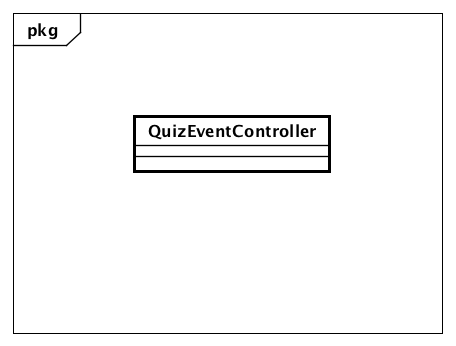
\includegraphics[scale=0.45]{UML/Classi/Front-End/QuizziPedia_Front-end_Controller_QuizEventController.png}
	\caption{QuizziPedia::Front-End::Controllers::QuizEventController}
\end{figure} \FloatBarrier
\begin{itemize}
	\item \textbf{Descrizione}: questa classe permette di reagire ai comandi dell'utente durante la gestione dei suoi questionari;
	\item \textbf{Utilizzo}: fornisce le funzionalità per reagire ai comandi dell'utente, effettua redirect alle pagine richieste, come la visualizzazione delle statistiche di un questionario e iniziare un questionario in modalità esame.
	\item \textbf{Relazione con altre classi}:
	\begin{itemize}
		\item \textit{IN} \texttt{CreationAndModifyDirective}:  
		\item \textit{OUT} \texttt{ExamModalityDirective}:
	\end{itemize}
	\item \textbf{Attributi}:
	\begin{itemize}
		\item \texttt{-} \texttt{\$scope: \$scope} \\
		Campo dati contenente un riferimento all’oggetto \$scope creato da \textit{Angular\ped{G}}, viene utilizzato come mezzo di comunicazione tra il controller e la view. Contiene gli oggetti che definiscono il model dell’applicazione;
	\end{itemize}
	\item \textbf{Metodi}:
	\begin{itemize}
		\item 
	\end{itemize}
\end{itemize}